% Options for packages loaded elsewhere
\PassOptionsToPackage{unicode}{hyperref}
\PassOptionsToPackage{hyphens}{url}
\PassOptionsToPackage{dvipsnames,svgnames,x11names}{xcolor}
%
\documentclass[
  11pt,
  bookmarksnumbered]{article}
\usepackage{amsmath,amssymb}
\usepackage{iftex}
\ifPDFTeX
  \usepackage[T1]{fontenc}
  \usepackage[utf8]{inputenc}
  \usepackage{textcomp} % provide euro and other symbols
\else % if luatex or xetex
  \usepackage{unicode-math} % this also loads fontspec
  \defaultfontfeatures{Scale=MatchLowercase}
  \defaultfontfeatures[\rmfamily]{Ligatures=TeX,Scale=1}
\fi
\usepackage{lmodern}
\ifPDFTeX\else
  % xetex/luatex font selection
\fi
% Use upquote if available, for straight quotes in verbatim environments
\IfFileExists{upquote.sty}{\usepackage{upquote}}{}
\IfFileExists{microtype.sty}{% use microtype if available
  \usepackage[]{microtype}
  \UseMicrotypeSet[protrusion]{basicmath} % disable protrusion for tt fonts
}{}
\makeatletter
\@ifundefined{KOMAClassName}{% if non-KOMA class
  \IfFileExists{parskip.sty}{%
    \usepackage{parskip}
  }{% else
    \setlength{\parindent}{0pt}
    \setlength{\parskip}{6pt plus 2pt minus 1pt}}
}{% if KOMA class
  \KOMAoptions{parskip=half}}
\makeatother
\usepackage{xcolor}
\usepackage[margin=1in]{geometry}
\usepackage{longtable,booktabs,array}
\usepackage{calc} % for calculating minipage widths
% Correct order of tables after \paragraph or \subparagraph
\usepackage{etoolbox}
\makeatletter
\patchcmd\longtable{\par}{\if@noskipsec\mbox{}\fi\par}{}{}
\makeatother
% Allow footnotes in longtable head/foot
\IfFileExists{footnotehyper.sty}{\usepackage{footnotehyper}}{\usepackage{footnote}}
\makesavenoteenv{longtable}
\usepackage{graphicx}
\makeatletter
\def\maxwidth{\ifdim\Gin@nat@width>\linewidth\linewidth\else\Gin@nat@width\fi}
\def\maxheight{\ifdim\Gin@nat@height>\textheight\textheight\else\Gin@nat@height\fi}
\makeatother
% Scale images if necessary, so that they will not overflow the page
% margins by default, and it is still possible to overwrite the defaults
% using explicit options in \includegraphics[width, height, ...]{}
\setkeys{Gin}{width=\maxwidth,height=\maxheight,keepaspectratio}
% Set default figure placement to htbp
\makeatletter
\def\fps@figure{htbp}
\makeatother
\setlength{\emergencystretch}{3em} % prevent overfull lines
\providecommand{\tightlist}{%
  \setlength{\itemsep}{0pt}\setlength{\parskip}{0pt}}
\setcounter{secnumdepth}{5}
\usepackage{titling}
\usepackage{pdfpages}
\usepackage{tocloft}
\usepackage{amsmath}
\usepackage{atbegshi}% http://ctan.org/pkg/atbegshi
\AtBeginDocument{\AtBeginShipoutNext{\AtBeginShipoutDiscard}}
\usepackage[spanish]{babel}
\usepackage{csquotes}
\usepackage{setspace}
\usepackage{float}
\floatplacement{figure}{H}
\usepackage[T1]{fontenc}
\usepackage[utf8]{inputenc}
\usepackage{fancyhdr}
\usepackage{hanging}
\usepackage{amsthm,amssymb,amsfonts}
\usepackage{tikz,lipsum,lmodern}
\usepackage{multicol}
\usepackage{fontawesome5}
\usepackage{multirow,booktabs,caption}
\usepackage{orcidlink}
\usepackage{anyfontsize}
\usepackage{geometry}
\geometry{bottom=1.2in }
\pagestyle{fancy}
\rhead{\textit{Comparativa de diferentes herramientas de visualización aplicados en big data}}
\definecolor{iacoldark}{RGB}{246, 127, 17}
\definecolor{iacol}{RGB}{131, 131, 131}
\usepackage{booktabs}
\usepackage{longtable}
\usepackage{array}
\usepackage{multirow}
\usepackage{wrapfig}
\usepackage{float}
\usepackage{colortbl}
\usepackage{pdflscape}
\usepackage{tabu}
\usepackage{threeparttable}
\usepackage{threeparttablex}
\usepackage[normalem]{ulem}
\usepackage{makecell}
\usepackage{xcolor}
\ifLuaTeX
  \usepackage{selnolig}  % disable illegal ligatures
\fi
\usepackage[]{biblatex}
\addbibresource{Referencias/Referencias.bib}
\IfFileExists{bookmark.sty}{\usepackage{bookmark}}{\usepackage{hyperref}}
\IfFileExists{xurl.sty}{\usepackage{xurl}}{} % add URL line breaks if available
\urlstyle{same}
\hypersetup{
  colorlinks=true,
  linkcolor={black},
  filecolor={Maroon},
  citecolor={blue},
  urlcolor={blue},
  pdfcreator={LaTeX via pandoc}}

\author{}
\date{\vspace{-2.5em}}

\begin{document}


\begin{center}
  \includepdf{portada.pdf}
\end{center}


\addtolength{\headheight}{1.4cm} 
\fancyhead[L]{
\includegraphics[width = 100pt]{logo.png}}
\renewcommand{\headrulewidth}{1pt}

{\normalsize
 \setcounter{tocdepth}{5}
 \tableofcontents
}


\newpage

\listoftables

\newpage

\listoffigures

\newpage

\begin{table}[H]
\centering
\caption{Lista de Abreviaturas} % Mover el título de la tabla arriba
\label{tab:abreviaturas}
\fontsize{12}{12}\selectfont % Especificar el tamaño de la fuente en puntos
\begin{tabular}{|l|l|}
\hline
\textbf{Abreviatura} & \textbf{Término} \\ \hline
API & Interfaz de Programación de Aplicaciones \\ \hline
API REST & Interfaz de Programación de Aplicaciones Representacional de Estado \\ \hline
AWS & Amazon Web Services \\ \hline
BDA & Big Data \& Analytics \\ \hline
BD & Big Data \\ \hline
BI & Inteligencia de Negocios \\ \hline
CPU & Unidad Central de Procesamiento \\ \hline
CRUD & Crear, Leer, Actualizar, Eliminar \\ \hline
CSV & Valores Separados por Comas \\ \hline
CSS & Hojas de Estilo en Cascada \\ \hline
DNS & Sistema de Nombres de Dominio \\ \hline
GPU & Unidad de Procesamiento Gráfico \\ \hline
GUI & Interfaz Gráfica de Usuario \\ \hline
HTML & Lenguaje de Marcado de Hipertexto \\ \hline
HTTP & Protocolo de Transferencia de Hipertexto \\ \hline
HTTPS & Protocolo Seguro de Transferencia de Hipertexto \\ \hline
IA & Inteligencia Artificial \\ \hline
IDE & Entorno de Desarrollo Integrado \\ \hline
IP & Protocolo de Internet \\ \hline
IoT & Internet de las cosas \\ \hline
JVM & Máquina Virtual de Java \\ \hline
JSON & Notación de Objetos JavaScript \\ \hline
LAN & Red de Área Local \\ \hline
M2M & Máquina a Máquina \\ \hline
ML & Aprendizaje Automático \\ \hline
MVC & Modelo-Vista-Controlador \\ \hline
NAT & Traducción de Direcciones de Red \\ \hline
ORACLE & Empresa de tecnología \\ \hline
PaaS & Plataforma como Servicio \\ \hline
RAM & Memoria de Acceso Aleatorio \\ \hline
RDBMS & Sistema de Gestión de Bases de Datos Relacionales \\ \hline
RA & Realidad Aumentada \\ \hline
RV & Realidad Virtual \\ \hline
SaaS & Software como Servicio \\ \hline
SDK & Kit de Desarrollo de Software \\ \hline
SQL & Lenguaje de consulta estructurado \\ \hline
SSL & Capa de Conexión Segura \\ \hline
TLS & Capa de Seguridad de Transporte \\ \hline
UI & Interfaz de Usuario \\ \hline
URL & Localizador Uniforme de Recursos \\ \hline
UX & Experiencia de Usuario \\ \hline
VPN & Red Privada Virtual \\ \hline
WAN & Red de Área Amplia \\ \hline
XML & Lenguaje de Marcado Extensible \\ \hline
CPF & Centro de procesamiento de fluidos de producción de petróleo \\ \hline
\end{tabular}
\end{table}

\newpage

\begin{center}
\textbf{Resumen}
\end{center}

\par
\begingroup
\leftskip1.5em
\rightskip\leftskip

Las herramientas de visualización de datos son fundamentales en la ciencia de datos y el análisis de Big Data, ya que ayudan a comprender, analizar y comunicar patrones complejos dentro de conjuntos masivos de datos.
Existen numerosas herramientas de visualización que varían en funcionalidades, capacidades de personalización, facilidad de uso y propósitos específicos.
Entre las más populares y utilizadas se encuentran: Tableau, Power BI, D3.js, Matplotlib, Seaborn, Plotly, Google Data Studio, QlikView/QlikSense, Grafana y ggplot2.

En la industria petrolera se generan grandes volúmenes de información diariamente en los diferentes procesos.
Se mantiene el registro de equipos, estrategias de mantenimiento preventivo, registro de fallas, documentación, ubicación de pozos, entre otros.
Por tanto, la visualización de datos desempeña un papel fundamental en este sector, permitiendo extraer, transformar y visualizar los datos de una manera sencilla y práctica.
Esto facilita la comprensión y detección de detalles importantes en la información, generando así un valor agregado para las empresas.

Este estudio realiza un análisis descriptivo de diversas herramientas disponibles en el mercado para la visualización de datos, evaluando sus diferencias, ventajas y desventajas.
Además, se presenta un caso práctico en el que se aplican las herramientas con mejor rendimiento para el sector, demostrando cómo los aspectos teóricos se reflejan en la práctica.
Para desarrollar este análisis, fue necesario investigar sobre tecnologías y herramientas para la visualización de grandes volúmenes de datos, explorar proyectos de BI en este sector y, finalmente, realizar una comparación para determinar en qué circunstancias una herramienta resulta más adecuada que otra para visualizar los datos de interés.

\textbf{Palabras clave}: Dashboard, Industria 4.0, sector petrolero, herramientas de visualización, Tableau, Power BI.

\newpage

\begin{center}
\textbf{abstract}
\end{center}

Data visualization tools are fundamental in data science and Big Data analysis, as they help to understand, analyze, and communicate complex patterns within massive data sets.
There are numerous visualization tools that vary in functionalities, customization capabilities, ease of use, and specific purposes.
Among the most popular and widely used are: Tableau, Power BI, D3.js, Matplotlib, Seaborn, Plotly, Google Data Studio, QlikView/QlikSense, Grafana, and ggplot2.

In the oil industry, large volumes of information are generated daily across various processes.
Records of equipment, preventive maintenance strategies, failure logs, documentation, well locations, among others, are maintained.
Therefore, data visualization plays a fundamental role in this sector, allowing data to be extracted, transformed, and visualized in a simple and practical manner.
This facilitates the understanding and detection of important details in the information, thus adding value to companies.

This study provides a descriptive analysis of various tools available in the market for data visualization, evaluating their differences, advantages, and disadvantages.
Additionally, a practical case is presented in which the best-performing tools for the sector are applied, demonstrating how theoretical aspects are reflected in practice.
To develop this analysis, it was necessary to research technologies and tools for visualizing large volumes of data, explore BI projects in this sector, and finally, make a comparison to determine under which circumstances one tool is better than another for visualizing the data of interest.

\textbf{Keywords}: Dashboard, Industry 4.0, oil sector, visualization tools, Tableau, Power BI.

\newpage

\hypertarget{introducciuxf3n}{%
\section{\texorpdfstring{\textbf{Introducción}}{Introducción}}\label{introducciuxf3n}}

La representación gráfica de cualquier información o dato se conoce como visualización de datos.
Esto ayuda a segregar los datos de manera eficiente mediante el uso de varios tipos de elementos visuales, como gráficos, mapas, tablas, mapas y herramientas de visualización.
Además de esto, con la ayuda de una herramienta de visualización de datos, los datos se pueden presentar de una manera única y comprensible para que las personas que no tienen experiencia técnica puedan entender todo fácilmente.

La visualización de datos es esencial para comunicar la información de manera efectiva, permitiendo a las personas comprender y analizar grandes cantidades de datos de manera más intuitiva y rápida.
Al representar los datos de manera visual, como a través de gráficos, mapas, diagramas y otros medios, se pueden identificar patrones, tendencias y relaciones que de otra manera pasan desapercibidos en conjuntos de datos complejos.

Además, la visualización de datos ayuda a revelar insights importantes, destacar anomalías o valores atípicos, respaldar la toma de decisiones fundamentadas en datos y contar historias con los datos.
Al proporcionar una representación visual clara y concisa de la información, las visualizaciones de datos permiten a los usuarios comprender la información de manera más rápida y efectiva, lo que facilita la extracción de conocimientos significativos y la formulación de acciones basadas en ellos.

La visualización de datos es esencial en la ciencia de datos y la arquitectura de presentación de datos.
Permite analizar patrones y relaciones en los datos, facilitando la extracción de conclusiones significativas.
Además, es crucial para monitorear el rendimiento de modelos de aprendizaje automático y análisis predictivos, interpretar resultados de manera accesible y comunicar hallazgos de manera efectiva a audiencias no técnicas.
En resumen, la visualización de datos es una herramienta fundamental para comprender, monitorear y comunicar resultados en diferentes contextos y aplicaciones.

Las herramientas de visualización de datos son esenciales para analizar y entender conjuntos de datos complejos.
Ofrecen interfaces intuitivas y diversas funcionalidades que permiten a los usuarios crear modelos visuales de datos de manera eficiente y personalizada.
Entre las razones de su popularidad se incluyen la facilidad de uso, la interactividad para explorar datos dinámicamente, la integración con bases de datos para importar y conectar datos fácilmente, y la inclusión de herramientas de aprendizaje automático para análisis predictivo.
Estas características hacen que estas herramientas sean ampliamente utilizadas por analistas, estadísticos y profesionales de datos para comunicar información de manera visual y accesible.

En el contexto de Big Data y ciencia de datos, las herramientas de visualización avanzada como Tableau, Power BI, D3.js y otras, permiten manejar y representar grandes conjuntos de datos de manera efectiva.
Estas herramientas facilitan la creación de paneles interactivos, gráficos geoespaciales, diagramas y modelos que ayudan a comprender mejor los datos complejos generados en el sector de hidrocarburos.
Por ende, este trabajo se enfoca en llevar a cabo una revisión bibliográfica que permita realizar investigaciones basadas en documentos, archivos y registros existentes.
El objetivo es responder a la pregunta acerca de la eficiencia de estas herramientas en el sector petrolero.
De manera que la visualización de datos en el sector de hidrocarburos no solo mejora la comprensión de los datos complejos, sino que también proporciona información clave para la toma de decisiones estratégicas, la optimización de procesos y la garantía de seguridad y sostenibilidad en la industria petrolera.

\hypertarget{objetivos}{%
\section{\texorpdfstring{\textbf{Objetivos}}{Objetivos}}\label{objetivos}}

Evaluar y comparar las soluciones de visualización de datos mas populares en el mercado, con un enfoque en su aplicación en el sector petrolero, analizando sus capacidades, fortalezas, limitaciones y adecuación para los requisitos específicos de la industria.

\hypertarget{objetivos-especuxedficos}{%
\subsection{Objetivos específicos}\label{objetivos-especuxedficos}}

• Investigar y comprender los requisitos y necesidades específicas de visualización de datos en el sector petrolero, incluyendo tipos de datos, volúmenes, formatos, análisis requeridos, entre otros.

• Definir un conjunto de criterios de evaluación relevantes para comparar las diferentes soluciones, considerando aspectos como capacidades de visualización, rendimiento, escalabilidad, integración con sistemas de información geográfica (GIS), soporte para formatos de datos geoespaciales, entre otros.

• Evaluar y calificar cada una de las soluciones identificadas en función de los criterios establecidos, analizando sus fortalezas, limitaciones y adecuación para los requisitos del sector petrolero.

• Elaborar un informe con los hallazgos incluyendo un caso práctico, conclusiones y recomendaciones del análisis comparativo, proporcionando una guía para la selección e implementación de la solución más adecuada en el sector petrolero.

• Identificar las principales herramientas y soluciones de visualización de datos, con enfoque geoespacial disponibles actualmente en el mercado.

\hypertarget{estado-del-arte-y-marco-teuxf3rico}{%
\section{\texorpdfstring{\textbf{Estado del arte y marco teórico}}{Estado del arte y marco teórico}}\label{estado-del-arte-y-marco-teuxf3rico}}

\hypertarget{introducciuxf3n-a-la-inteligencia-de-negocios}{%
\subsection{Introducción a la Inteligencia de Negocios}\label{introducciuxf3n-a-la-inteligencia-de-negocios}}

La inteligencia de negocios se puede definir como un conjunto de herramientas y soluciones tecnológicas diseñadas para que los usuarios puedan extraer de manera eficiente información empresarial útil, para apoyar y soportar el proceso de toma de decisiones, obteniendo una ventaja competitiva sobre otras organizaciones.
De acuerdo con \textcite{xu2007research}.
La BI ha evolucionado a lo largo de varias décadas impulsada por el progreso tecnológico y la creciente necesidad de las organizaciones de tomar decisiones informadas basadas en datos.
Los orígenes de la BI se remontan a los años sesenta, cuando se desarrollaron los primeros sistemas de información gerencial (MIS, por sus siglas en inglés) y los sistemas de soporte de decisiones (DSS).

Por otra parte, otros autores importantes confirman estos hechos, por citar algunos como \textcite{tutunea2012business} quienes en su artículo describen que los primeros pasos hacia BI se dieron a principios de la década de 1960, cuando se introdujo el concepto de sistemas de información gerencial y las primeras aplicaciones de soporte de decisiones.
Estos sistemas iniciales tenían capacidades limitadas y se enfocaban principalmente en la recopilación y presentación de datos estructurados, y en 1970 el concepto data warehouse, introducido por IBM, fue un gran impulsor para el desarrollo de la inteligencia de negocios.

De acuerdo con la historia en los años ochenta y noventa, con la expansión de las computadoras personales y el desarrollo de herramientas de visualización de datos y reporting impulsaron la adopción de BI en las empresas.
La aparición de técnicas de minería de datos y análisis avanzado amplió las capacidades de BI para esas épocas.
En la era moderna, la BI ha experimentado una transformación significativa impulsada por la explosión de datos, la computación en la nube y la integración con tecnologías emergentes como el aprendizaje automático y la inteligencia artificial.

De acuerdo a \textcite{jourdan2008business}, la integración de BI con herramientas de minería de datos y técnicas de inteligencia artificial ha permitido un análisis más sofisticado y una toma de decisiones más informada'' (p.~122), esta se convertido en una herramienta indispensable para las organizaciones que buscan mantenerse competitivas en un entorno empresarial cada vez más impulsado por los datos y es un factor clave para el éxito empresarial, ya que permite a las organizaciones aprovechar al máximo sus recursos de información y tomar decisiones estratégicas basadas en datos.

Para el presente, estas herramientas son una pieza clave para la toma de decisiones en las organizaciones empresariales, permiten la recolección, extracción, integración y análisis y presentación de los datos, facilitando la interpretación, análisis de tendencias, patrones y demás operaciones con datos que ayudan a la eficiencia operativa de la empresa.
Esta importancia radica en la capacidad para transformar grandes volúmenes de datos en información valiosa, lo que conlleva a la toma decisiones informadas, mejorar la eficiencia operativa y obtener una ventaja competitiva en el mercado o sector industrial.
Por otra parate también resaltar que las herramientas, como Tableau, Power BI y QlikView, ofrecen interfaces intuitivas y visualizaciones avanzadas, haciendo que el análisis de datos sea accesible para usuarios con diversos niveles de experiencia técnica.

\hypertarget{visualizaciuxf3n-de-grandes-voluxfamenes-de-datos.}{%
\subsection{Visualización de grandes volúmenes de datos.}\label{visualizaciuxf3n-de-grandes-voluxfamenes-de-datos.}}

La era actual dominada por la información, los datos abundan tanto estructurados como no estructurados.
Estos datos, si se analizan y comprenden correctamente, pueden revelar patrones ocultos, tendencias significativas y conocimientos valiosos que pueden transformar diversos aspectos cotidianos.
La visualización de datos implica representar información y datos numéricos utilizando elementos visuales como gráficos, tablas y mapas.
Este proceso transforma conjuntos de datos, ya sean grandes o pequeños, en imágenes que resultan accesibles y comprensibles para las personas \textcite{javatpoint2023data}.

La importancia de la visualización de grandes volúmenes de datos radica en su capacidad para revelar información valiosa a partir de conjuntos de datos complejos y multidimensionales.
Esta información o datos, pueden impulsar a la toma de decisiones informadas que contribuye a mejorar la eficiencia operativa, identificar oportunidades de negocio y promover la innovación en la empresa \textcite{shneiderman1996eyes}.
Por otra parte, una visualización efectiva de datos facilita la comunicación y la colaboración entre diferentes equipos y partes interesadas, al presentar la información de manera intuitiva y accesible.

Uno de los principales poderes de la visualización de grandes volúmenes de datos es su capacidad para revelar patrones y tendencias que podrían pasar desapercibidos en representaciones numéricas o tabulares.
Al aprovechar la capacidad humana para procesar información visual, las técnicas de visualización permiten identificar rápidamente anomalías, agrupaciones y relaciones complejas dentro de los datos \textcite{few2009now}.

Otra ventaja significativa de la visualización de grandes volúmenes de datos es su capacidad para manejar conjuntos de datos de diferentes fuentes y formatos.
Mediante la integración y transformación de datos estructurados y no estructurados, las herramientas de visualización pueden crear representaciones unificadas y coherentes, lo que facilita el análisis y la interpretación \textcite{ware2012information}.
Esto es particularmente relevante en entornos donde se manejan datos de diversas fuentes, como en la industria del big data y la analítica avanzada.

En el campo del Big Data de acuerdo con diferentes estudios por citar una herramienta como Power BI, donde se resalta la capacidad para conectarse a una amplia gama de fuentes de datos, tanto locales como en la nube, le permite integrar y analizar grandes volúmenes de información provenientes de diversas fuentes.
De acuerdo con \textcite{aspin2019high}, ``Power BI puede manejar conjuntos de datos masivos de hasta varios terabytes, lo que lo convierte en una opción viable para el análisis de Big Data en entornos empresariales'' (p.~142).
Además, Power BI cuenta con funciones avanzadas de modelado de datos y visualización, lo que permite a los usuarios explorar y comprender patrones y tendencias complejas en los datos de manera intuitiva y significativa.

\hypertarget{datos-en-el-sector-petrolero.}{%
\subsection{Datos en el sector petrolero.}\label{datos-en-el-sector-petrolero.}}

El sector petrolero es uno de los pilares fundamentales de la economía global, siendo responsable de la producción y distribución de una de las fuentes de energía más importantes del mundo, el petróleo y la Industria Petrolera en Colombia es fuerte, se considera que es un actor significativo en la industria petrolera global, aunque no se encuentra entre los mayores productores del mundo, su papel es crucial tanto para su economía nacional como para el mercado energético global.
A continuación, se presenta un análisis detallado de la producción petrolera de Colombia.

Colombia ocupa el puesto 22 a nivel mundial en términos de producción de petróleo, con una producción diaria que ha oscilado entre 700,000 y 900,000 barriles por día (bpd) en los últimos años \textcite{bp2023statistical}.
Este nivel de producción lo posiciona como el cuarto mayor productor de petróleo en América Latina, después de Brasil, México y Venezuela.
En cuanto a las reservas probadas de petróleo, Colombia cuenta con aproximadamente 1.8 mil millones de barriles.
Estas reservas, aunque modestas en comparación con gigantes como Venezuela o Arabia Saudita, son esenciales para mantener la producción y asegurar la autosuficiencia energética del país a corto y mediano plazo \textcite{bp2023statistical}.

En este contexto planteado, los datos y la generación de datos juegan un papel crucial para optimizar operaciones, mejorar la seguridad y maximizar la eficiencia operativa de la empresa.
Necesidad que ha llevado a la implementación de tecnologías avanzadas y a la adopción de sistemas de gestión de datos sofisticados que transforman grandes volúmenes de información en conocimientos importantes para la empresa, ahora en temas de mantenimiento industrial es importante mantener los equipos operativos para evitar pérdidas de producción y accidentes catastróficos que de echo han ocurrido en la industria.

Por tanto, que datos se pueden encontrar en el sector petrolero, a continuación, se hace una lista de la información clave en este sector.

\begin{enumerate}
\def\labelenumi{\arabic{enumi}.}
\item
  Información de equipos industriales: En este punto entran todos los equipos industriales que se manejan en la empresa, como: Generadores, turbinas, Baterías, Aires, Instrumentos, Paneles solares, Motores eléctricos ect.
\item
  Estrategia de mantenimiento:~ Corresponde a todos los planes de mantenimiento que se le hace a cada uno de los equipos, esta se conoce como el plan de mantenimiento preventivo.
\item
  Datos Mantenimiento Correctivo:~ Corresponde a toda la información de mantenimiento correctivo que se le hace a los equipos, este mantenimiento se hace por solicitud y también se puede dar que muchos equipos tenga una estrategia de mantenimiento a falla que se puede considerar como mantenimiento correctivo.
\item
  Materiales: Corresponde a la información de los materiales y repuestos que se requieren para la atención de los diferentes equipos presentes en las facilidades.
\item
  Ordenes De trabajo: Corresponde a las órdenes de trabajo que se generan para atender los equipos, las ordenes de trabajo pueden ser preventivas cuando nacen de un plan de mantenimiento correctivas cuando se hacen por una falla presente en el equipo industrial.
\item
  Costos: Todo lo relacionado a costos del mantenimiento, los costos de mantenimiento se basan en tiempos o mano de obra y costos de repuestos asicados a la relación.
\item
  Compras: Las compras son registros en especial para adquirir repuestos para los equipos, estas compras se asocian a un orden de trabajo y antes de hacer la compra debe existir una reserva.
\item
  Otros: También se maneja información de proveedores, reparaciones a edificios y parte civil como vías, información de procesos de integridad e inventarios de metrología entre otros procesos propios de la industria que generan gran cantidad de datos día a día.
\end{enumerate}

Por otra parte en este sector es importante cumplir y mantener los equipos en buenas condiciones para evitar incidentes que pongan en riesgo la integridad de la planta y las personas, de acuerdo \textcite{ortiz2021importancia} la implementación de KPI`s permite a las empresas petroleras no solo monitorear su desempeño en tiempo real, sino también realizar ajustes oportunos que pueden prevenir costos adicionales y mejorar la calidad de los procesos.
Según un estudio de la Universidad Pontificia Bolivariana, el sector oil \& gas en Colombia ha sido pionero en la adopción de KPIs debido a su utilidad en la gestión y optimización de operaciones.

Algunos KPIs que se manejan en este sector:

\begin{enumerate}
\def\labelenumi{\arabic{enumi}.}
\tightlist
\item
  \textbf{Ready Backlog}: El término ``Ready Backlog'' se refiere a la carga de trabajo pendiente de tareas de mantenimiento que están listas para ser ejecutadas. Se trata de un concepto importante para garantizar la planificación y ejecución eficiente del mantenimiento preventivo y correctivo. Este Indicador mide la carga de trabajo en semanas que se encuentra registrada en SAP para cada Equipo de trabajo, el Target esta de 4 a 6 semana. Horas Hombre Planeadas (Ordenes de Trabajo) / Horas Hombre Disponibles (Capacidad laboral de acuerdo con los técnicos que se tienen para ejecutar los mantenimientos).
\end{enumerate}

\begin{figure}

{\centering 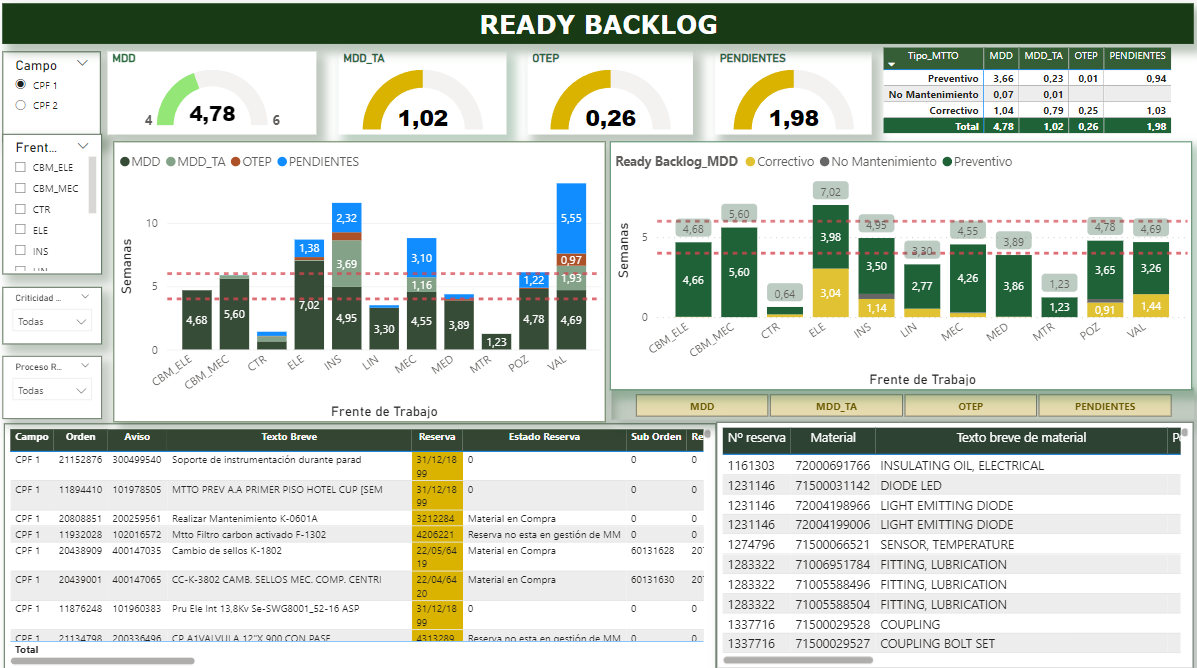
\includegraphics[width=5.98in]{media/image2} 

}

\caption{Panel de control de la dashboard en Power BI, llamada Ready Baclog. Fuente: Propia}\label{fig:unnamed-chunk-1}
\end{figure}

\begin{enumerate}
\def\labelenumi{\arabic{enumi}.}
\setcounter{enumi}{1}
\tightlist
\item
  \textbf{Cumplimiento Estrategia de Mantenimiento}: Es un indicador que mide el cumplimiento de los planes preventivos en periodo de tiempo mensual, la estrategia puede ser crítica y no critica.
\end{enumerate}

\begin{figure}

{\centering 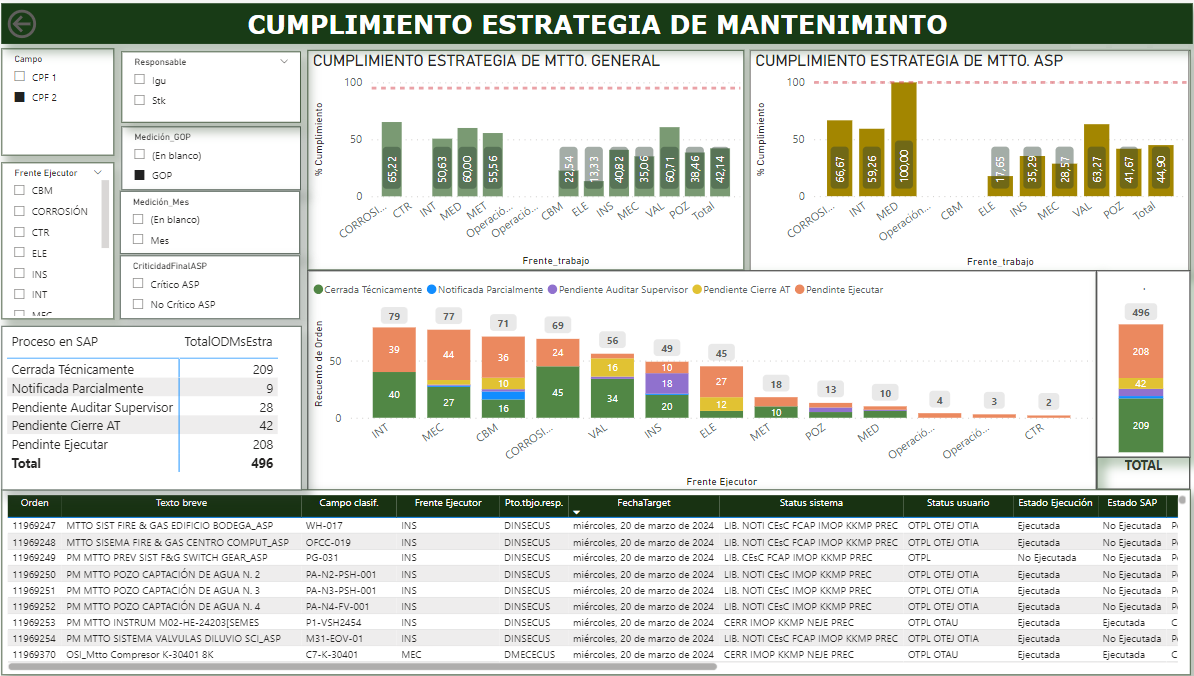
\includegraphics[width=4.78in]{media/image3} 

}

\caption{Cumplimento de la estrategia de mantenimiento en Power BI. Fuente: Propia}\label{fig:unnamed-chunk-2}
\end{figure}

\newpage

\begin{enumerate}
\def\labelenumi{\arabic{enumi}.}
\setcounter{enumi}{2}
\item
  \textbf{Producción diaria de petróleo}: Este KPI mide la cantidad de barriles de petróleo producidos por día.
  Es fundamental para monitorear la eficiencia de la producción y detectar cualquier desviación respecto a las metas establecidas.
\item
  \textbf{Tasa de recuperación de reservas}: Indica el porcentaje de petróleo recuperado de un yacimiento en relación con el total de reservas disponibles.
  Es crucial para evaluar la efectividad de las técnicas de extracción utilizadas.
\item
  \textbf{Costos operativos por barril}: Este indicador mide los costos asociados a la producción de un barril de petróleo, incluyendo gastos en exploración, perforación, extracción y transporte.
  Ayuda a las empresas a controlar sus costos y mejorar la rentabilidad.
\item
  \textbf{Tiempo de inactividad no planificado}: Mide el tiempo en el que la producción se detiene debido a fallas imprevistas o mantenimiento no planificado.
  Minimizar este tiempo es esencial para mantener una producción constante y eficiente.
\item
  \textbf{Índice de incidentes de seguridad}: Evalúa la cantidad y gravedad de los incidentes de seguridad que ocurren en las operaciones petroleras.
  Un alto índice puede indicar la necesidad de mejorar las prácticas de seguridad y capacitación.
\item
  \textbf{Tasa de éxito en exploración}: Mide el porcentaje de proyectos de exploración que resultan en descubrimientos comercialmente viables.
  Este KPI es importante para evaluar la efectividad de las actividades de exploración y la capacidad de la empresa para identificar nuevas reservas.
\end{enumerate}

\hypertarget{impacto-de-las-herramientas-bi-en-la-eficiencia-operativa.}{%
\subsection{Impacto de las herramientas BI en la eficiencia Operativa.}\label{impacto-de-las-herramientas-bi-en-la-eficiencia-operativa.}}

En el entorno empresarial actual y más en el sector petrolero, la toma de decisiones basada en datos ha adquirido una gran importancia.
Las empresas y organizaciones industriales se enfrentan a desafíos constantes, como la optimización de procesos, la reducción de costos y el aumento de la eficiencia operativa.
En este contexto, las herramientas de Inteligencia de Negocios BI, han surgido como una solución poderosa para ayudar a las empresas a aprovechar al máximo sus datos y mejorar su eficiencia operativa, ya que entre muchos procesos permiten a las organizaciones recolectar, analizar y visualizar datos de manera que se pueda tomar decisiones informadas y estratégicas.

De acuerdo con \textbf{Wayne Eckerson}, \textcite{eckerson2010performance} en su libro sobre rendimiento de dashboard, señala que uno de los principales beneficios de las herramientas BI es su capacidad para visualizar los datos de manera intuitiva y comprensible.
Los cuadros de mando interactivos y los informes personalizados permiten a los usuarios explorar y comprender los datos de manera más efectiva, lo que facilita la identificación de cuellos de botella, ineficiencias y oportunidades de optimización.
Estas afirmaciones son parte del uso que se le dan a estas herramientas la actualidad no solo la capacidad de análisis también se resalta la vista o diseño que genera un atractivo a la hora de presentar los datos o KPIs.
Por otra parte, el autor resalta un aspecto importante y es la capacidad de las herramientas BI para integrar datos de diferentes fuentes y departamentos dentro de una empresa industrial.
Esto permite una visión más completa y precisa de las operaciones, lo que facilita la identificación de áreas de mejora y la toma de decisiones.

Para el caso de información geoespacial, estas herramientas también tienen un gran potencial y han demostrado ser invaluables en esta tarea, ofreciendo a las organizaciones la oportunidad de localizar puntos críticos en diferentes sectores y tomar medidas correctivas basadas en datos, en el sector petrolero existen los pozos de producción donde se generan datos y una de las ventajas es poder identificar cada pozo en un mapa de la región y analizar los datos puntuales para estos, tema que un herramienta BI se puede realizar con facilidad pero que resulta de gran ayuda para el sector petrolero.

\hypertarget{marco-teuxf3rico}{%
\section{\texorpdfstring{\textbf{Marco Teórico}}{Marco Teórico}}\label{marco-teuxf3rico}}

\hypertarget{big-data-y-las-herramientas-de-visualizaciuxf3n.}{%
\subsection{Big Data y las herramientas de visualización.}\label{big-data-y-las-herramientas-de-visualizaciuxf3n.}}

A pesar de que el término ``Big Data'' es reciente, los antecedentes de los enormes conjuntos de datos se remontan a las décadas de 1960 y 1970, cuando el campo de la gestión de datos estaba en sus primeras etapas, con la aparición de los primeros centros de datos y el desarrollo de las bases de datos relacionales \textcite{oracle2023big}.

Cuando las organizaciones comenzaron a utilizar computadoras para almacenar y analizar grandes cantidades de datos.
Sin embargo, no fue hasta finales de la década de 1990 y principios de la de 2000 que el análisis de Big Data realmente comenzó a despegar, a medida que las organizaciones recurrieron cada vez más a las computadoras para ayudarlas a dar sentido a los volúmenes de datos en rápido crecimiento que generan sus negocios.
\textcite{simplilearn2023big}.

El concepto de utilizar imágenes se lanzó en el siglo XVII para comprender los datos de mapas y gráficos y luego, a principios del siglo XIX, se reinventó en el gráfico circular.
\textcite{javatpoint2023data} Las primeras herramientas de visualización de datos se utilizaron en el siglo XVII para representar datos económicos y demográficos.
En el siglo XIX, se desarrollaron herramientas más sofisticadas para representar datos científicos, como los gráficos de líneas y de barras.
En el siglo XX, las herramientas de visualización de datos se utilizaron cada vez más en los negocios y la industria.
Las empresas comenzaron a utilizarlas para representar datos financieros, de ventas y de producción \textcite{wainer2022origins}.

La visualización de datos para la interpretación de datos existe desde el comienzo de la civilización.
Mediante el uso de la visualización de datos, las personas podían comprender el mundo en el que vivían y hacer predicciones más precisas sobre eventos futuros \textcite{helical2023data}.

• 1644: El astrólogo femenino Michael Florent van Langren proporcionó la primera representación de datos estadísticos.

• 1700: Surgió el mapeo temático y se introdujeron gráficos abstractos de funciones, errores de medición y recopilación de datos empíricos.

• 1800: William Playfair introdujo algunos de los gráficos más utilizados.

• 1854: El médico John Snow mapea el brote de cólera en Londres en un gráfico.

• Principios de 1900: La visualización de datos comienza a ganar publicidad y los gráficos comienzan a aparecer cada vez más en libros, revistas, etc.

• Finales de 1900: El avance del procesamiento y almacenamiento informático permitió almacenar, procesar y analizar una cantidad cada vez mayor de datos.

• Década de 1960-1970: Los investigadores John Tukey y Jacques Bertin desarrollan la ciencia de la visualización de datos en estadística y cartografía.

• Principios de la década de 1980: Edward Tufte publica ``La visualización de información cuantitativa'', que se utiliza actualmente en las universidades.

Las computadoras hicieron posible procesar una gran cantidad de datos a velocidades vertiginosas.
Hoy en día, la visualización de datos se convierte en una combinación de arte y ciencia en rápida evolución que seguramente cambiará el panorama corporativo en los próximos años.

\begin{figure}

{\centering 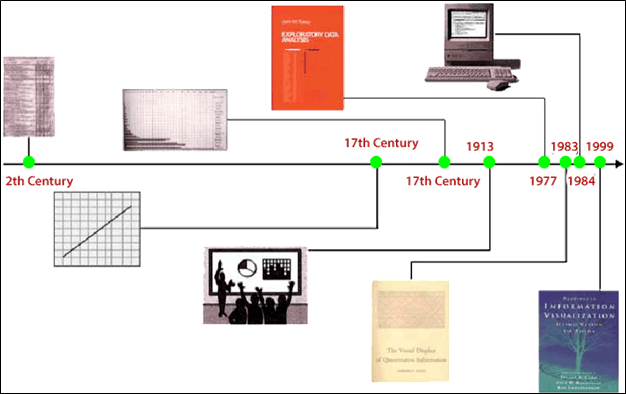
\includegraphics[width=3.13in]{media/image4} 

}

\caption{Historia de la visualización de los grandes datos. Fuente: (Java T Point, 2023)}\label{fig:unnamed-chunk-3}
\end{figure}

El desarrollo de las tecnologías de big data en la década de 1990 dio lugar a un nuevo auge en el campo de la visualización de datos.
Las herramientas de visualización de big data están diseñadas para manejar grandes volúmenes de datos, lo que las hace ideales para aplicaciones en el sector empresarial, la investigación científica y el gobierno \textcite{olshannikova2016visualizing}.

La herramienta de visualización de Big data están empezando a integrar la inteligencia artificial y el aprendizaje automático para automatizar tareas, como la selección de datos y la creación de visualizaciones.
Las herramientas de visualización de big data están empezando a utilizar la realidad aumentada y la realidad virtual para crear experiencias de visualización más inmersivas.
Las herramientas de visualización de big data están empezando a centrarse en la visualización de datos en tiempo real para permitir a los usuarios tomar decisiones más informadas en tiempo real \textcite{schwabish2021better}.

\hypertarget{cuxf3mo-funcionan-las-herramientas-de-grandes-datos.}{%
\subsection{Cómo funcionan las herramientas de grandes datos.}\label{cuxf3mo-funcionan-las-herramientas-de-grandes-datos.}}

Las herramientas de visualización de datos funcionan mediante la conexión con diferentes fuentes de datos, la transformación de esos datos en visualizaciones interactivas y la presentación de la información de manera comprensible y útil.

\textbf{Power BI} permite la conexión con diversas fuentes de datos, como bases de datos, archivos locales, servicios en la nube, entre otros.
Los datos se importan o se conectan en tiempo real, se pueden transformar y modelar según las necesidades del usuario.
Luego, se crean visualizaciones (gráficos, tablas, mapas, etc.) que se organizan en un panel de control interactivo.
Estos paneles se pueden compartir y colaborar en tiempo real \textcite{microsoft2023powerbi}.

\textbf{Tableau} permite la conexión con múltiples fuentes de datos, donde se extraen, limpian y transforman los datos.
Los usuarios pueden arrastrar y soltar elementos visuales para crear paneles interactivos.
Utiliza un enfoque ``arrastrar y soltar'' para la creación de visualizaciones avanzadas y también permite la exploración de datos en tiempo real \textcite{tableau2023effective}.

\textbf{Qlik} utiliza un enfoque de ``asociación de datos'' para crear visualizaciones.
Los datos se cargan en memoria y se modelan asociativamente, lo que permite a los usuarios explorar libremente la información y descubrir relaciones entre los datos de forma dinámica.
Las visualizaciones se actualizan automáticamente cuando se realiza un cambio en los datos \textcite{qlik2023difference}.

\textbf{Google Data Studio}: Google Data Studio se conecta a una variedad de fuentes de datos, incluidos servicios de Google como Google Analytics, Google Ads, entre otros.
Permite la creación de informes interactivos arrastrando y soltando componentes visuales.
Los datos se actualizan automáticamente y los informes se pueden compartir fácilmente con otros usuarios \textcite{looker2023support}.

\textbf{D3.js}: D3.js es una biblioteca JavaScript que permite la creación de visualizaciones de datos personalizadas.
Funciona manipulando el DOM de un navegador web para generar gráficos interactivos a partir de datos.
Los usuarios pueden crear gráficos altamente personalizados mediante la codificación de las interacciones y elementos visuales deseados \textcite{d3js2023d3}.

El proceso general de visualización de grandes datos con estas herramientas se puede dividir en los siguientes pasos:

\begin{enumerate}
\def\labelenumi{\arabic{enumi}.}
\item
  \textbf{Recopilación de datos}: El primer paso es recopilar los datos que se van a visualizar.
  Los datos pueden provenir de una variedad de fuentes, como bases de datos, archivos y aplicaciones.
\item
  \textbf{Preparación de datos}: Una vez recopilados los datos, es necesario prepararlos para la visualización.
  Esto puede implicar limpiar los datos, eliminar valores atípicos y transformar los datos en un formato que sea compatible con la herramienta de visualización.
\item
  \textbf{Visualización}: El siguiente paso es crear las visualizaciones.
  Las visualizaciones pueden ser simples o complejas, y pueden utilizar una variedad de gráficos y tablas.
\item
  \textbf{Análisis}: Una vez creadas las visualizaciones, se pueden utilizar para analizar los datos.
  El análisis puede ayudar a identificar tendencias, patrones y anomalías.
\item
  \textbf{Comunicación}: Las visualizaciones se pueden utilizar para comunicar los resultados del análisis a otros.
  Las visualizaciones pueden ser efectivas para comunicar información compleja de una manera clara y concisa.
\end{enumerate}

Estas herramientas utilizan diferentes enfoques y métodos para transformar datos en visualizaciones comprensibles, lo que permite a los usuarios explorar, analizar y comunicar la información de manera efectiva.

\hypertarget{herramientas-de-visualizaciuxf3n-de-grandes-datos}{%
\subsection{Herramientas de visualización de grandes datos}\label{herramientas-de-visualizaciuxf3n-de-grandes-datos}}

\hypertarget{tableu.}{%
\subsubsection{Tableu.}\label{tableu.}}

Es líder del mercado de canales de análisis de big data.
Las empresas lo utilizan para publicar visualizaciones de datos de alta calidad.
Tableau Desktop admite cientos de opciones de importación de datos, desde archivos CSV hasta API para una integración completa con AWS, Spark, Hadoop, Microsoft SQL y más.
La versión empresarial admite fuentes de datos en vivo para paneles de BI.
Tableau Public es la versión gratuita para uso personal: sus creaciones son públicas y solo se pueden guardar en la nube.
También está limitado a extraer datos de CSV, Excel y otros archivos planos \textcite{upwork2023best}.

\hypertarget{microsoft-powerbi}{%
\subsubsection{Microsoft PowerBI}\label{microsoft-powerbi}}

Es líder de la industria en plataformas de análisis e inteligencia empresarial.
Sus conectores de datos facilitan la extracción de datos de otras aplicaciones y se integra muy bien con todas las fuentes habituales de análisis de big data (por ejemplo, AWS, Spark y Hadoop).
Es una opción natural si su pila de tecnología empresarial ya utiliza tecnologías de Microsoft.
El modelo de suscripción anual premium también proporciona recursos de almacenamiento y computación en la nube dedicados \textcite{upwork2023best}.

se posiciona como una herramienta poderosa para conectar, extraer y analizar datos de una amplia gama de fuentes.
Desde bases de datos y servicios en la nube hasta hojas de cálculo y más, Power BI permite a los usuarios transformar datos sin procesar en información significativa a través de un conjunto completo de funciones.
Facilita la conexión y extracción de datos desde diversas fuentes, como bases de datos, servicios en la nube y hojas de cálculo, entre otras.
Ofrece una amplia gama de representaciones visuales interactivas, como gráficos, tablas dinámicas y mapas.
Los usuarios tienen la capacidad de construir tableros personalizados que combinan múltiples visualizaciones en una sola página.
Además, proporciona herramientas para limpiar y transformar datos, simplificando así la preparación de los mismos para el análisis.
Emplea el lenguaje DAX (Data Analysis Expressions) para realizar cálculos y crear medidas personalizadas.

\hypertarget{fusioncharts}{%
\subsubsection{FusionCharts}\label{fusioncharts}}

Es un paquete de visualización de datos basado en JavaScript.
Puede comprar licencias con ofertas según el tamaño de su equipo de desarrollo.
Como paquete de JavaScript en lugar de una herramienta, tiene la máxima flexibilidad para crear paneles de control públicos y privados para manejar el procesamiento de big data.
Un diferenciador clave es la extensa biblioteca de plantillas en vivo de FusionCharts: simplemente conecte sus datos y véalos visualizados al instante \textcite{upwork2023best}.

Ofrece una amplia gama de tipos de gráficos, desde gráficos de barras y gráficos circulares hasta mapas geográficos y medidores.
Los usuarios pueden explorar datos, hacer clic en elementos para obtener detalles y realizar acciones específicas según la configuración.

Se integra fácilmente en aplicaciones web y de escritorio mediante código HTML, JavaScript y otras tecnologías web estándar.
Es compatible con una amplia variedad de tecnologías y marcos, incluidos Angular, React, JavaScript puro y otros.
Los gráficos se pueden personalizar para adaptarse a las necesidades de diseño y marca de una aplicación o sitio web.
Los desarrolladores pueden ajustar colores, fuentes y más.
Pueden conectarse a datos dinámicos, lo que permite la actualización en tiempo real de las visualizaciones en función de los cambios en los datos subyacentes.

\hypertarget{google-data-studio}{%
\subsubsection{Google Data Studio}\label{google-data-studio}}

Google Data Studio es gratuito, pero quienes lo utilicen para empresas probablemente tendrán que pagar por una conexión de datos a un servicio como Supermetrics.
La plataforma es para analistas de negocios que pueden conocer un poco de programación con Python o JavaScript y desean generar informes y elementos visuales para paneles \textcite{upwork2023best}.
Permite conectar y extraer datos de una variedad de fuentes, incluyendo Google Analytics, Google Ads, Google Sheets, bases de datos SQL, archivos CSV entre otros.
Los usuarios pueden crear informes personalizados que incluyen gráficos, tablas, imágenes y texto.
Los informes pueden personalizarse en términos de estilo y formato para que coincidan con la marca de una empresa o proyecto.

\hypertarget{flourish}{%
\subsubsection{Flourish}\label{flourish}}

Es popular entre los periodistas que desean contar historias con datos.
Su interfaz de usuario intuitiva facilita que los no codificadores recopilen y presenten datos en visualizaciones de datos pulidas y compatibles con dispositivos móviles.
La interfaz se ejecuta en el navegador y le permite ajustar el ancho y el estilo de su objeto visual de datos a medida que lo crea para ver cómo se vería con diferentes anchos de pantalla.
También permite a los desarrolladores crear plantillas personalizadas con su SDK de desarrollador \textcite{upwork2023best}.

Ofrece una amplia variedad de visualizaciones interactivas, que incluyen gráficos de barras, gráficos de líneas, mapas, gráficos de dispersión y más.
Se destaca la creación de visualizaciones sin necesidad de codificación ni experiencia en diseño gráfico.
Los usuarios pueden importar datos desde una variedad de fuentes, incluyendo hojas de cálculo, archivos CSV, bases de datos en línea y más.
También se pueden utilizar integraciones con servicios como Google Sheets.

\hypertarget{sisense}{%
\subsubsection{Sisense}\label{sisense}}

Sisense es una plataforma de análisis de datos y Business Intelligence (BI) que permite a las organizaciones recopilar, analizar y visualizar datos para tomar decisiones informadas y estratégicas.
Es una plataforma de análisis de datos de un extremo a otro con una interfaz empresarial que cualquier analista de BI reconocerá.
Se puede implementar localmente o en la nube y proporciona visualizaciones de datos sólidas para informes y paneles \textcite{upwork2023best}.
Es utilizado por empresas de diversas industrias para el análisis de datos, la generación de informes y la toma de decisiones estratégicas.
Su enfoque en la facilidad de uso y la capacidad de análisis avanzado lo convierten en una opción popular para aquellos que buscan implementar soluciones de Business Intelligence en sus operaciones comerciales.

\hypertarget{chartblocks}{%
\subsubsection{ChartBlocks}\label{chartblocks}}

Es un creador de gráficos en línea fácil de usar que le permite crear visualizaciones de datos personalizadas sin conocimientos de programación.
La plataforma también facilita compartir e insertar gráficos en sitios web y redes sociales.
Construidas a partir de D3.js, las visualizaciones de ChartBlocks responden y se representan como archivos SVG con buena presentación en pantallas de alta resolución \textcite{upwork2023best}.

\hypertarget{qlik-sense}{%
\subsubsection{Qlik Sense}\label{qlik-sense}}

Desarrollado sobre el motor asociativo de Qlik, Qlik Sense le permite encontrar conexiones y comprender claramente la información al convertir datos sin procesar en visualizaciones atractivas.
Puede utilizar Qlik Sense para realizar análisis estadísticos y crear interfaces de usuario flexibles, tablas dinámicas y gráficos, entre otras funciones.
Si recopila datos de múltiples fuentes, Qlik Sense le permite fusionar los datos en una nueva tabla para facilitar el análisis \textcite{upwork2023best}.

En general, Qlik Sense es una plataforma de BI potente y versátil que se puede utilizar para analizar datos y tomar mejores decisiones.
Es una buena opción para empresas de todos los tamaños y para personas que desean aprovechar al máximo sus datos.

\hypertarget{datawrapper}{%
\subsubsection{Datawrapper}\label{datawrapper}}

Ya sea que esté creando tablas responsivas, visualizaciones interactivas o mapas, Datawrapper proporciona herramientas para ayudar a contar una historia.
Tiene un plan gratuito que puedes usar para crear, publicar y exportar visualizaciones, pero solo puedes descargar el contenido en formato PNG.
No necesita ningún conocimiento especial para trabajar con Datawrapper y puede importar datos desde archivos CSV y XLS o copiarlos y pegarlos en el editor de Datawrapper \textcite{upwork2023best}.
Ofrece una extensa variedad de tipos de gráficos y representaciones visuales, que abarcan desde gráficos de barras y líneas hasta gráficos de dispersión, mapas, tablas y más.
Su principal destacado radica en la capacidad de los usuarios para crear visualizaciones de datos sin necesidad de poseer conocimientos avanzados en diseño gráfico o programación.
La herramienta permite personalizar la apariencia de las visualizaciones, incluyendo opciones como colores, etiquetas, títulos y fuentes.
Facilita la importación de datos desde diversas fuentes, como hojas de cálculo, archivos CSV y bases de datos en línea, e incluso es compatible con datos en tiempo real.
Además, las visualizaciones creadas con Datawrapper son responsivas, adaptándose automáticamente a diferentes tamaños de pantalla, lo que las convierte en una opción idónea para su inclusión en sitios web y presentaciones.

\newpage

\hypertarget{metodologuxeda}{%
\section{\texorpdfstring{\textbf{Metodología}}{Metodología}}\label{metodologuxeda}}

Para el desarrollo de este caso práctico, se empleó la metodología CRISP-DM (Cross Industry Standard Process for Data Mining), ampliamente reconocida en el ámbito de la minería de datos \textcite{shearer2000crispdm}.
Esta metodología se complementó con el método jerárquico AHP (Analytic Hierarchy Process) para evaluar y seleccionar la herramienta de BI (Business Intelligence) más adecuada según los criterios definidos.

\hypertarget{fases-de-crisp-dm}{%
\subsubsection{Fases de CRISP-DM}\label{fases-de-crisp-dm}}

\begin{enumerate}
\def\labelenumi{\arabic{enumi}.}
\item
  \textbf{Comprensión del Negocio}: En esta fase, se identificaron los objetivos y requisitos del negocio para definir el problema a resolver \textcite{wirth2000crispdm}.
\item
  \textbf{Comprensión de los Datos}: Se recopiló y exploró la información relevante para el análisis.
\item
  \textbf{Preparación de los Datos}: Incluyó la limpieza y transformación de los datos para adecuarlos al análisis.
\item
  \textbf{Modelado}: Se aplicaron técnicas de análisis de datos para construir modelos predictivos.
\item
  \textbf{Evaluación}: Los modelos se evaluaron para asegurar que cumplen con los objetivos del negocio.
\item
  \textbf{Despliegue}: Los modelos finales se implementaron en el entorno de producción.
\end{enumerate}

La metodología CRISP-DM (Cross-Industry Standard Process for Data Mining) proporciona una estructura sistemática para guiar el desarrollo del caso práctico.

\begin{figure}

{\centering 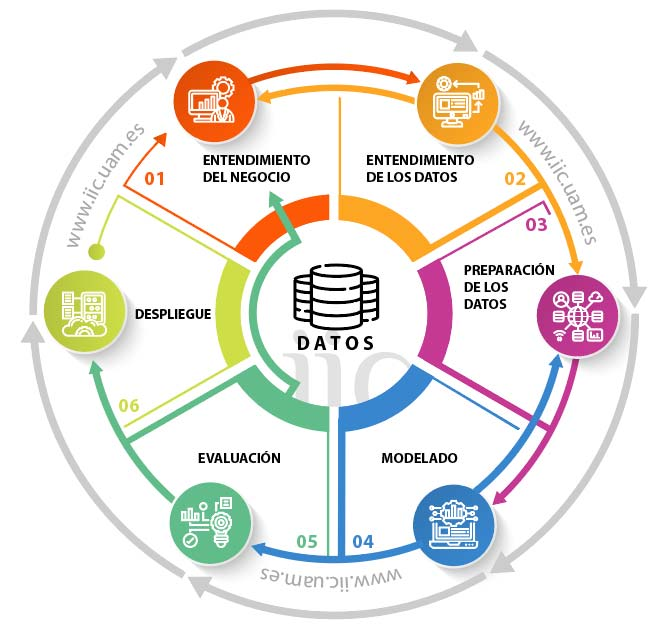
\includegraphics[width=3.28in]{media 2/image1} 

}

\caption{Metodologia Crips-DM}\label{fig:unnamed-chunk-4}
\end{figure}

\hypertarget{aplicaciuxf3n-del-muxe9todo-ahp}{%
\subsubsection{Aplicación del Método AHP}\label{aplicaciuxf3n-del-muxe9todo-ahp}}

La Metodología del Proceso Analítico Jerárquico (AHP) es una técnica de toma de decisiones multicriterio desarrollada por Thomas L. Saaty en la década de 1970 \textcite{saaty1980analytic}.

Es ampliamente utilizada para resolver problemas complejos que implican múltiples criterios y alternativas.
AHP descompone un problema de decisión en una jerarquía de subproblemas más manejables, cada uno de los cuales puede ser analizado de manera independiente.

\hypertarget{pasos-principales-en-ahp}{%
\subsubsection{Pasos Principales en AHP}\label{pasos-principales-en-ahp}}

\begin{enumerate}
\def\labelenumi{\arabic{enumi}.}
\item
  \textbf{Definición del Problema y Construcción de la Jerarquía:}

  \begin{itemize}
  \item
    \textbf{Nivel 1:} Objetivo principal del problema.
  \item
    \textbf{Nivel 2:} Criterios que influyen en la decisión.
  \item
    \textbf{Nivel 3:} Subcriterios (si los hay) y alternativas posibles.
  \end{itemize}
\item
  \textbf{Comparaciones Pareadas:}

  \begin{itemize}
  \tightlist
  \item
    Realizar comparaciones entre los criterios y las alternativas en pares, utilizando una escala de 1 a 9 para evaluar su importancia relativa.
  \end{itemize}
\item
  \textbf{Cálculo de los Pesos Relativos:}

  \begin{itemize}
  \tightlist
  \item
    Normalizar las matrices de comparación pareada y calcular los pesos promedios para cada criterio y subcriterio.
  \end{itemize}
\item
  \textbf{Síntesis de los Resultados:}

  \begin{itemize}
  \tightlist
  \item
    Combinar los pesos de los criterios con los pesos de las alternativas para obtener un puntaje global para cada alternativa.
  \end{itemize}
\item
  \textbf{Verificación de la Consistencia:}

  \begin{itemize}
  \tightlist
  \item
    Evaluar la consistencia de las comparaciones para asegurar que las decisiones sean razonables y no arbitrarias.
  \end{itemize}
\end{enumerate}

El método AHP se utilizó para evaluar diversas herramientas de BI con base en los siguientes criterios:

\begin{itemize}
\item
  \textbf{Conectividad y Fuentes de Datos}: La capacidad de la herramienta para conectarse a diversas fuentes de datos \textcite{saaty1980analytic}.
\item
  \textbf{Capacidades de Transformación}: Facilidad y potencia en la transformación de datos.
\item
  \textbf{Seguridad}: Características de seguridad y control de acceso.
\item
  \textbf{Geolocalización}: Capacidades de análisis y visualización geoespacial.
\item
  \textbf{Interfaz de Usuario}: Usabilidad y diseño de la interfaz.
\item
  \textbf{Rendimiento y Escalabilidad}: Capacidad de manejar grandes volúmenes de datos y escalabilidad.
\item
  \textbf{Soporte y Comunidad}: Disponibilidad de soporte técnico y comunidad de usuarios.
\item
  \textbf{Coste y Licenciamiento}: Costes asociados a la implementación y mantenimiento de la herramienta.
\end{itemize}

La combinación de CRISP-DM y AHP permitió una evaluación estructurada y objetiva, asegurando que se seleccionara la herramienta de BI más adecuada para las necesidades específicas del proyecto.

\hypertarget{comprensiuxf3n-del-negocio}{%
\subsection{Comprensión del Negocio}\label{comprensiuxf3n-del-negocio}}

Para el caso práctico se tiene como objetivo comparar dos herramientas de visualización de datos, Power BI y Google Data Studio, en el contexto de un caso práctico donde se desarrollaron tableros de mando para monitorear el KPI de Productividad.
Para la gestión de mantenimiento, es importante el monitoreo de la productividad laboral y la identificación de oportunidades de mejora con tiempos improductivos mediante el análisis de la información, con el objetivo de enfocar la mano de obra en la ejecución de las actividades de mantenimiento y optimizar los tiempos improductivos que se generan.

Productividad en el contexto del mantenimiento y operaciones en la industria petrolera se refiere a la eficiencia con la que los recursos (humanos, financieros, materiales) se utilizan para generar resultados.
En particular, se mide a través de los tiempos productivos y no productivos, buscando oportunidades de mejora para optimizar los tiempos de reparación y mitigar o eliminar malos actores (Campbell, Jardine, \& McGlynn, 2011; Balmer, 1999).

\begin{enumerate}
\def\labelenumi{\arabic{enumi}.}
\item
  \textbf{Tiempos Productivos o Hands On}: Se refiere al tiempo que los trabajadores dedican directamente a las tareas de mantenimiento y operación sobre los equipos.
  Es un indicador clave para evaluar la eficiencia laboral y la utilización de los recursos humanos.
  Se busca que los tiempos productivos Hands On sean superiores a los tiempos improductivos No Hands On.
\item
  \textbf{Tiempos Improductivos o No Hands On}: Se refiere al tiempo que no se dedica directamente a las tareas productivas, incluyendo reuniones, desplazamientos a sitios de trabajo, esperas por materiales o equipos, alistamiento de equipos y otras actividades que no contribuyen directamente a la producción o mantenimiento efectivo sobre el equipo.
  Se busca optimizar estos tiempos mediante el análisis de lo ocurrido y la formulación de planes de acción que mitiguen o eliminen estas afectaciones.
  Dentro de los tiempos improductivos se discrimina el porcentaje asociado a temas de capacitaciones, charlas y actividades de salud ocupacional que se denominan ``Actividades Generales''.
\end{enumerate}

En el sector petrolero la productividad está dada por:

\textbf{Productividad = {[}Hora Hombre ejecutadas en trabajo efectivo en el equipo{]} / {[}Total de Horas Hombre Ejecutadas{]}}

\begin{itemize}
\item
  \textbf{Hands On:} Porcentaje de Horas Empleadas en actividades puntuales de mantenimiento en los Equipos o activos industriales.
  Este es igual a la productividad.
\item
  \textbf{No Hands On:} Porcentaje de Horas Empleadas en actividades que apoyan la ejecución de las actividades, dentro de estas tenemos:
\end{itemize}

\begin{enumerate}
\def\labelenumi{\arabic{enumi}.}
\tightlist
\item
  Apertura permiso de trabajo
\item
  Documentos (Diligencia de Check List, ART, Reporte ODM)~~~~~~~~~~
\item
  Herramientas / Materiales~~~~~~~~~~~~~~~~~~~~~~~~~~
\item
  Aislamiento \& Des aislamiento de Proceso~~~~~~~~~~~~~~~~~~~~~~~~~
\item
  Aislamiento \& Des aislamiento Eléctrico~~~~~~~~~~~~~~~~~~~~~~~~~~~~
\item
  Charla es sitio~~~~~~~~~~~~~~~~~~~~~~~
\item
  Movilización a sitio
\item
  Espera necesaria (por trabajos interdisciplinarios / simultáneos)~~
\item
  Descanso Auditivo / Valoraciones Medicas
\item
  Causas Externas (lluvia, alarma, etc.)
\item
  Tiempos Desplazamiento \& Alistamientos Alimentación
\end{enumerate}

\begin{itemize}
\tightlist
\item
  \textbf{Actividades Generales:} Porcentaje de Horas Empleadas en actividades de:
\end{itemize}

\begin{enumerate}
\def\labelenumi{\arabic{enumi}.}
\item
  Salud Ocupacional
\item
  Reunión de supervisores diaria
\item
  Actividades de Recursos Humanos
\item
  Capacitaciones y Charlas
\item
  Actividades de Bienestar
\end{enumerate}

\hypertarget{comprensiuxf3n-de-los-datos}{%
\subsection{Comprensión de los datos}\label{comprensiuxf3n-de-los-datos}}

El conjunto de datos que se utilizara para la comparativa entre herramientas de visualización comprende dos set de datos con la información de la gestión de Mantenimiento, un set de datos con la información geoespacial de los centros de acopio o (CPF), un set de datos que permite la conversión de los nombres de los puestos o frentes de trabajo en abreviaturas esto para ocupar menos espacio en pantalla en las gráficas y mejorar así la visualización, un set de datos con la descripción de los códigos de productividad.

\begin{figure}

{\centering 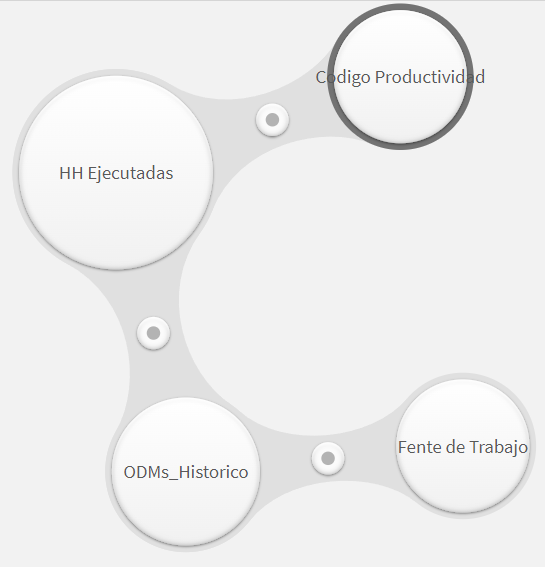
\includegraphics[width=2.72in]{media 2/image2} 

}

\caption{Metodologia Crips-DM}\label{fig:unnamed-chunk-5}
\end{figure}

\hypertarget{bases-de-datos-principales}{%
\subsubsection{Bases de datos Principales}\label{bases-de-datos-principales}}

\textbf{Dataset 1: Histórico Gestión de Mantenimiento Ordenes de trabajo}

\begin{table}[H]

\caption{\label{tab:unnamed-chunk-6}Histórico Gestión de Mantenimiento Ordenes de trabajo}
\centering
\fontsize{9}{11}\selectfont
\begin{tabular}[t]{l|>{\raggedright\arraybackslash}p{35em}}
\hline
Variable & Descripcion\\
\hline
Orden & Número Único con el que se identifica una actividad de Mantenimiento sobre un Activo Industrial\\
\hline
Texto breve & Descripción de la actividad que se va a ejecutar sobre el Activo Industrial\\
\hline
Aviso & Número Único con el que se reporta una falla y que dará inicio a la creación de una Orden de trabajo\\
\hline
Campo de clasificación & Tag o Nombre del Activo Industrial\\
\hline
Fecha de referencia & Fecha de planificación de la Orden de trabajo\\
\hline
Pto.tbjo.responsable & Frente de trabajo (Mecánico, Eléctrico, Instrumentación, Válvulas, Procesos) al que le corresponde ejecutar las actividades de mantenimiento\\
\hline
Status de usuario & Estado, Planificación y Programación de la Orden de trabajo en SAP, Orden Liberada, Orden en proceso de Planificación, Orden Pendiente Materiales, Orden Pendiente Terceros, Orden Pendiente Parada Planta\\
\hline
Status del sistema & Estado del sistema de la Orden de trabajo en SAP, Orden Abierta, Orden Ejecutada, Orden Cerrada\\
\hline
Criticidad ASP & ASP (Aseguramiento por Seguridad de Procesos) se clasifican los equipos en críticos por ASP (S), No Críticos, no Aplica criticidad\\
\hline
Clase de orden & Código que identifica el origen de la orden de trabajo si proviene de un Plan de mantenimiento o de un reporte correctivo\\
\hline
Clase actividad PM & Clasificación de la actividad Preventiva, Correctiva, Predictiva\\
\hline
Centro emplazamiento & Número único asociado al campo petrolero\\
\hline
Emplazamiento & Número Único asociado a una área específica del campo petrolero\\
\hline
CeCo responsable & Centro de costo asociado al frente de trabajo ejecutor (Eléctrico, Mecánico, Instrumentación)\\
\hline
Centro de coste & Centro de Costos asociado al Activo Industrial dependiendo su naturaleza\\
\hline
Costes tot.reales & Costos Totales de la ejecución de la actividad de Mantenimiento\\
\hline
\end{tabular}
\end{table}

\newpage

\textbf{Histórico Horas Hombre ejecutadas en Ordenes de trabajo para la Gestión de Mantenimiento.}

Está conformado por 80.4187 Observaciones y 4 Variables.

\begin{table}[H]

\caption{\label{tab:unnamed-chunk-7}Histórico Horas Hombre ejecutadas en Ordenes de trabajo para la Gestión de Mantenimiento.}
\centering
\fontsize{9}{11}\selectfont
\begin{tabular}[t]{l|>{\raggedright\arraybackslash}p{35em}}
\hline
Variable & Descripcion\\
\hline
Orden & Número Único con el que se identifica una actividad de Mantenimiento sobre un Activo Industrial\\
\hline
Puesto trabajo (real) & Frente de trabajo (Mecánico, Eléctrico, Instrumentación, Válvulas, Pozos) al que le corresponde ejecutar las actividades de mantenimiento\\
\hline
Trabajo real & Horas Hombre Ejecutadas\\
\hline
Texto de notificación & Código Productividad que permite la distribución de las horas hombre ejecutadas (Horas Empleadas en trabajo efectivo sobre la máquina, Horas empleadas en Permisos de trabajo, Horas empleadas en Movilizaciones entre otras actividades.)\\
\hline
\end{tabular}
\end{table}

\hypertarget{bases-de-datos-de-apoyo}{%
\subsubsection{Bases de datos de apoyo}\label{bases-de-datos-de-apoyo}}

\textbf{Códigos de Productividad}

\begin{table}[H]

\caption{\label{tab:unnamed-chunk-8}Códigos de Productividad}
\centering
\fontsize{9}{11}\selectfont
\begin{tabular}[t]{l|>{\raggedright\arraybackslash}p{35em}}
\hline
Variable & Descripcion\\
\hline
CodPro & Llave que clasifica las actividades ejecutadas y que permita la distribución de las horas hombre ejecutadas clasificándolas en actividades productivas y tiempos muertos.\\
\hline
Des.CodPro & Descripción detallada del código de productividad. Esta información es importante para el proceso de análisis que se haga.\\
\hline
\end{tabular}
\end{table}

\textbf{Puestos de Trabajo}

\begin{table}[H]

\caption{\label{tab:unnamed-chunk-9}Puestos de Trabajo}
\centering
\fontsize{9}{11}\selectfont
\begin{tabular}[t]{l|>{\raggedright\arraybackslash}p{35em}}
\hline
Variable & Descripcion\\
\hline
PT & Llave con la que se identifica el puesto de trabajo, este está asociado a la disciplina dueña de la actividad de mantenimiento (Eléctrica, Mecánica, Instrumentación, etc.)\\
\hline
Recurso & Es una abreviación del PT (Puesto de Trabajo) Ej: ELE = Electricidad\\
\hline
Empresa & Nombre de la Empresa a la que está asociado el puesto de trabajo\\
\hline
\end{tabular}
\end{table}

\hypertarget{preparaciuxf3n-de-los-datos}{%
\subsection{Preparación de los datos}\label{preparaciuxf3n-de-los-datos}}

Para asegurar que la visualización de los datos permita tomar decisiones adecuadas en la gestión de mantenimiento, es necesario garantizar una adecuada limpieza y transformación de datos.
De ahí la importancia de que la herramienta seleccionada para la visualización de los datos sea robusta en este aspecto.

\hypertarget{histuxf3rico-gestiuxf3n-de-mantenimiento-ordenes-de-trabajo}{%
\subsubsection{Histórico Gestión de Mantenimiento Ordenes de Trabajo}\label{histuxf3rico-gestiuxf3n-de-mantenimiento-ordenes-de-trabajo}}

\textbf{Campo Orden:} Este campo es muy importante ya que se convierte en la llave que permite relacionarse con la información de la tabla ``Histórico Horas Hombre ejecutadas en Ordenes de Trabajo para la Gestión de Mantenimiento''.
Se debe asegurar que en ambas tablas no contengan elementos vacíos.

\textbf{Campo Criticidad ASP:} Para este campo, los registros nulos corresponden a equipos que no requieren evaluación de criticidad.
Por lo tanto, para efectos del informe se consideran dentro de la población de equipos No Críticos por seguridad de proceso y no se deben eliminar.
Con base en la información de este campo se crea la columna ``Criticidad ASP'' así:

\begin{itemize}
\item
  Si el valor es ``S'', asignar ``Crítico ASP''
\item
  Si no, asignar ``No Crítico ASP''
\end{itemize}

\textbf{Campo Centro Emplazamiento:} La información de este campo es la llave que permite el enlace con la información de la tabla que contiene Latitudes y Longitudes de los campos Petroleros (CPF), permitiendo la visualización geoespacial.
Con base en la información de este campo se crea la columna ``Campo'' así:

\begin{itemize}
\item
  Si el valor es ``1063'', asignar ``Campo A''
\item
  Si el valor es ``1064'', asignar ``Campo B''
\end{itemize}

\textbf{Campo ``Puesto Responsable'':} La información de este campo es la llave que permite el enlace con la información de la tabla ``Frente de Trabajo'' que contiene una abreviación del nombre al que hace referencia el puesto de trabajo y la Empresa a la que pertenece.

\hypertarget{historico-de-horas-para-la-gestion-de-mantenimiento}{%
\subsubsection{Historico de Horas para la gestion de Mantenimiento}\label{historico-de-horas-para-la-gestion-de-mantenimiento}}

\textbf{Campo Orden:} Este campo es muy importante ya que se convierte en la llave que permite relacionarse con la información de la tabla ``Histórico Gestión de Mantenimiento Ordenes de Trabajo''.
Se debe asegurar que en ambas tablas no contengan elementos vacíos.

\textbf{Campo Texto de Notificación:} La información de este campo es la llave que permite el enlace con la información de la tabla ``Código Productividad'' para obtener una descripción detallada del código.
Además, con la información de este campo se construirá la columna ``Productividad'' para distribuir las Horas Hombre ejecutadas en:

\begin{itemize}
\item
  \textbf{Actividades Hands On:} Horas Hombre trabajo efectivo sobre la máquina o equipo.
\item
  \textbf{Actividades No Hands On:} Horas Hombre empleadas en trabajo de alistamiento para ejecutar la actividad (e.g., apertura de permisos de trabajo, alistamiento de herramientas).
\item
  \textbf{Actividades Generales:} Horas Hombre empleadas en actividades de capacitación, charlas, actividades de bienestar.
\end{itemize}

Registros nulos se eliminan del conjunto de datos.

\textbf{Campo Trabajo Real:} Este campo contiene las Horas Hombre ejecutadas distribuidas por los códigos de productividad.
Los registros vacíos se deben eliminar ya que no serían representativos al sumar las Horas Hombre y realizar la distribución de productividad.

\hypertarget{generaciuxf3n-de-columnas-calculadas}{%
\subsubsection{Generación de Columnas Calculadas}\label{generaciuxf3n-de-columnas-calculadas}}

\textbf{Productividad:} Este campo permite la clasificación de productividad de las horas hombre ejecutadas.

\begin{itemize}
\item
  Algoritmo:

  \begin{itemize}
  \item
    Si ``Texto de notificación'' es igual a ``HSO'', Productividad igual ``Hands On''.
  \item
    Si ``Texto de notificación'' es igual a ``ALB'', Productividad igual ``Actividades Generales''.
  \item
    Si no, Productividad igual ``No Hands On''.
  \end{itemize}
\end{itemize}

\textbf{Campo:} De acuerdo al ``Centro Emplazamiento'' se clasifica el centro de acopio del campo petrolero.

\begin{itemize}
\item
  Algoritmo:

  \begin{itemize}
  \item
    Si ``Centro Emplazamiento'' es igual a ``1063'', Campo igual ``Cusiana''.
  \item
    Si ``Centro Emplazamiento'' es igual a ``1064'', Campo igual ``Cupiagua''.
  \item
    Si no, Campo igual ``Sin Clasificar''.
  \end{itemize}
\end{itemize}

\textbf{Ciudad:} De acuerdo al ``Centro Emplazamiento'' se clasifica el centro de acopio del campo petrolero.

\begin{itemize}
\item
  Algoritmo:

  \begin{itemize}
  \item
    Si ``Centro Emplazamiento'' es igual a ``1063'', Ciudad igual ``Tauramena''.
  \item
    Si ``Centro Emplazamiento'' es igual a ``1064'', Ciudad igual ``Aguazul''.
  \item
    Si no, Campo igual ``Sin Clasificar''.
  \end{itemize}
\end{itemize}

\textbf{Latitud:} De acuerdo al ``Centro Emplazamiento'' se asocia la Latitud.

\begin{itemize}
\item
  Algoritmo:

  \begin{itemize}
  \item
    Si ``Centro Emplazamiento'' es igual a ``1063'', Latitud igual ``5.00094378666''.
  \item
    Si ``Centro Emplazamiento'' es igual a ``1064'', Latitud igual ``5.20993248812''.
  \end{itemize}
\end{itemize}

\textbf{Longitud:} De acuerdo al ``Centro Emplazamiento'' se asocia la Longitud.

\begin{itemize}
\item
  Algoritmo:

  \begin{itemize}
  \item
    Si ``Centro Emplazamiento'' es igual a ``1063'', Longitud igual ``-72.7062007108''.
  \item
    Si ``Centro Emplazamiento'' es igual a ``1064'', Longitud igual ``-72.60170928352''.
  \end{itemize}
\end{itemize}

\textbf{Año:} Se extrae el Año del campo ``Fecha de referencia''.

\begin{itemize}
\tightlist
\item
  Algoritmo: Año (``Fecha de referencia'').
\end{itemize}

\textbf{Mes:} Se extrae el Mes del campo ``Fecha de referencia''.

\begin{itemize}
\tightlist
\item
  Algoritmo: Mes (``Fecha de referencia'').
\end{itemize}

\hypertarget{generaciuxf3n-de-medidas}{%
\subsubsection{Generación de Medidas}\label{generaciuxf3n-de-medidas}}

\textbf{Cálculo Tiempos Hands On (Tiempos efectivos de trabajo sobre la máquina):}

\begin{itemize}
\item
  Medida ``Hands\_On'': Sumatoria ``Trabajo Real'' (Horas Hombre ejecutadas) donde ``Texto de notificación'' sea igual a ``HSO''.
\item
  Medida ``\% Hands\_On'': Horas Hombre Hands On dividido entre el total de horas ejecutadas.
\end{itemize}

\textbf{Cálculo Tiempos Actividades Generales (Tiempos empleados en reuniones, capacitaciones):}

\begin{itemize}
\item
  Medida ``Actividades Generales'': Sumatoria ``Trabajo Real'' (Horas Hombre ejecutadas) donde ``Texto de notificación'' sea igual a ``ALB''.
\item
  Medida ``\% Actividades Generales'': Horas Hombre Actividades Generales dividido entre el total de horas ejecutadas.
\end{itemize}

\textbf{Cálculo Tiempos No Hands On (Tiempos improductivos):}

\begin{itemize}
\item
  Medida ``No Hands\_On'': Sumatoria ``Trabajo Real'' (Horas Hombre ejecutadas) donde ``Texto de notificación'' no sea (``HSO'', ``ALB'').
\item
  Medida ``\% No\_Hands\_On'': Horas Hombre No Hands On dividido entre el total de horas ejecutadas.
\end{itemize}

\hypertarget{modelado}{%
\subsection{Modelado}\label{modelado}}

Se desarrolla tableros de visualización en Power BI, Qlik Cloud y Looker Studio, en esta fase de desarrollo se presenta una evaluación del comportamiento de cada una de las herramientas con respecto a cada característica que se tendrá en cuenta para definir que herramienta de visualización es la más adecuada para la implementación de los KPIs, la experiencia obtenida en el desarrollo de este caso práctico apoyara el juicio para la asignasion de la puntuación en las matrices de evaluación de acuerdo a la metodología AHP (Analytic Hierarchy Process).

\hypertarget{conectividad-y-fuentes-de-datos}{%
\subsubsection{Conectividad y Fuentes de Datos}\label{conectividad-y-fuentes-de-datos}}

\hypertarget{fuentes-de-datos-y-capacidades-de-integraciuxf3n-en-el-sector-petrolero}{%
\paragraph{Fuentes de Datos y Capacidades de Integración en el Sector Petrolero}\label{fuentes-de-datos-y-capacidades-de-integraciuxf3n-en-el-sector-petrolero}}

En el sector petrolero, las empresas manejan datos de múltiples fuentes, incluyendo almacenamientos en la nube, bases de datos y archivos planos generados por softwares de monitoreo de equipos.
Es clave la capacidad de conexión a diversas fuentes de datos, ya que permite a la empresa adaptarse rápidamente a cambios en sus sistemas de información.
En el desarrollo del caso práctico se evidenciaron las siguientes capacidades:

\begin{enumerate}
\def\labelenumi{\arabic{enumi}.}
\item
  \textbf{Fuentes de Datos Soportadas}:

  \begin{itemize}
  \item
    \textbf{Pregunta}: ¿Cuántas y qué tipo de fuentes de datos pueden conectarse directamente (bases de datos, servicios en la nube, archivos planos, etc.)?
  \item
    \textbf{Descripción}: Es crucial evaluar la variedad de fuentes de datos que la herramienta puede soportar, ya que esto determina su flexibilidad y adaptabilidad en un entorno con múltiples orígenes de datos.
  \end{itemize}
\item
  \textbf{Conectividad en Tiempo Real}:

  \begin{itemize}
  \item
    \textbf{Pregunta}: ¿Permite la conectividad en tiempo real para algunas fuentes de datos?
  \item
    \textbf{Descripción}: La conectividad en tiempo real es fundamental para asegurar que la información sea actual y precisa, lo que permite una toma de decisiones más rápida y efectiva.
  \end{itemize}
\item
  \textbf{Capacidades de Integración}:

  \begin{itemize}
  \item
    \textbf{Pregunta}: ¿Qué tan bien se integran con otras herramientas y servicios que ya están en uso en la organización?
  \item
    \textbf{Descripción}: La capacidad de integración con otros sistemas y herramientas existentes en la organización mejora la eficiencia operativa y facilita la adopción de la herramienta.
  \end{itemize}
\end{enumerate}

\hypertarget{caso-pruxe1ctico-uso-de-power-bi-en-el-sector-petrolero}{%
\paragraph{Caso Práctico: Uso de Power BI en el Sector Petrolero}\label{caso-pruxe1ctico-uso-de-power-bi-en-el-sector-petrolero}}

En el desarrollo del caso práctico, se evidenció la capacidad de Power BI Desktop para conectarse a datos de diferentes orígenes, lo que lo convierte en una herramienta atractiva para la implementación de visualizaciones en el sector petrolero.

\hypertarget{conectividad-y-fuentes-de-datos-en-power-bi-desktop}{%
\paragraph{Conectividad y Fuentes de Datos en Power BI Desktop}\label{conectividad-y-fuentes-de-datos-en-power-bi-desktop}}

Power BI Desktop permite conectarse a una amplia variedad de fuentes de datos, incluyendo:

\begin{itemize}
\item
  Bases de datos
\item
  Servicios en la nube
\item
  Archivos planos
\end{itemize}

Esta capacidad es particularmente útil en el sector petrolero, donde se manejan múltiples fuentes de datos.
Durante el caso práctico, Power BI se integró eficazmente con otros softwares de Microsoft que la empresa ya tenía implementados, como SharePoint y Office.
Además, se realizaron conexiones con Google Drive y SharePoint para demostrar la versatilidad y capacidad de integración de Power BI.

\begin{figure}

{\centering 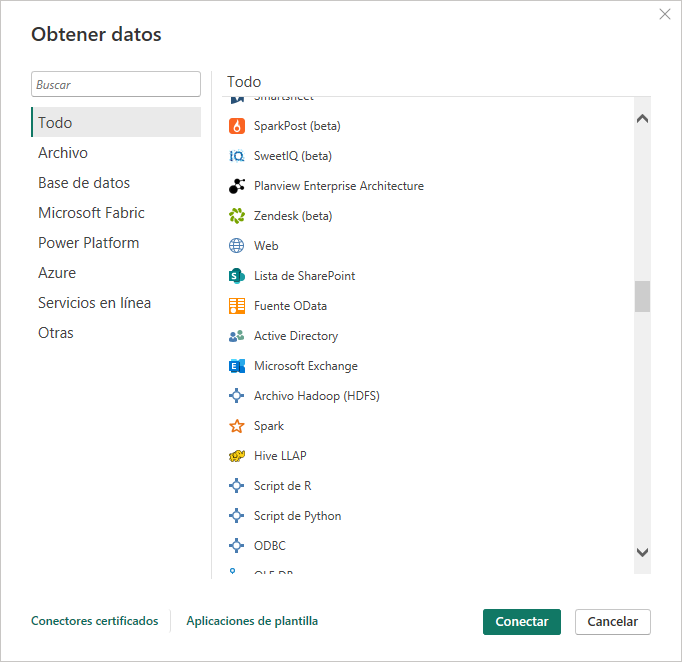
\includegraphics[width=3.41in]{media 2/image6} 

}

\caption{Tipos de archivos que pueden cargarse a Power BI}\label{fig:unnamed-chunk-10}
\end{figure}

\hypertarget{caso-pruxe1ctico-uso-de-qlik-cloud-en-el-sector-petrolero}{%
\paragraph{Caso Práctico: Uso de Qlik Cloud en el Sector Petrolero}\label{caso-pruxe1ctico-uso-de-qlik-cloud-en-el-sector-petrolero}}

Durante el caso práctico, Qlik Cloud demostró su capacidad para incorporar datos a una plataforma en la nube o replicar datos desde diversas fuentes.
Esta versatilidad permite a la empresa adaptarse rápidamente a cambios en sus sistemas de información, mejorando la eficiencia operativa y la toma de decisiones.

\hypertarget{conectividad-y-fuentes-de-datos-en-qlik-cloud}{%
\paragraph{Conectividad y Fuentes de Datos en Qlik Cloud}\label{conectividad-y-fuentes-de-datos-en-qlik-cloud}}

Qlik Cloud permite la integración con una gran cantidad de fuentes de datos, incluyendo:

\begin{itemize}
\tightlist
\item
  Aplicaciones SaaS
\item
  Bases de datos
\item
  Almacenes de datos en la nube
\item
  SAP HANA
\end{itemize}

Esta capacidad es particularmente útil en el sector petrolero, donde se manejan múltiples fuentes de datos.
La conexión directa con SAP HANA es especialmente interesante, ya que el software para la gestión de mantenimiento utilizado es precisamente SAP.

\begin{figure}

{\centering 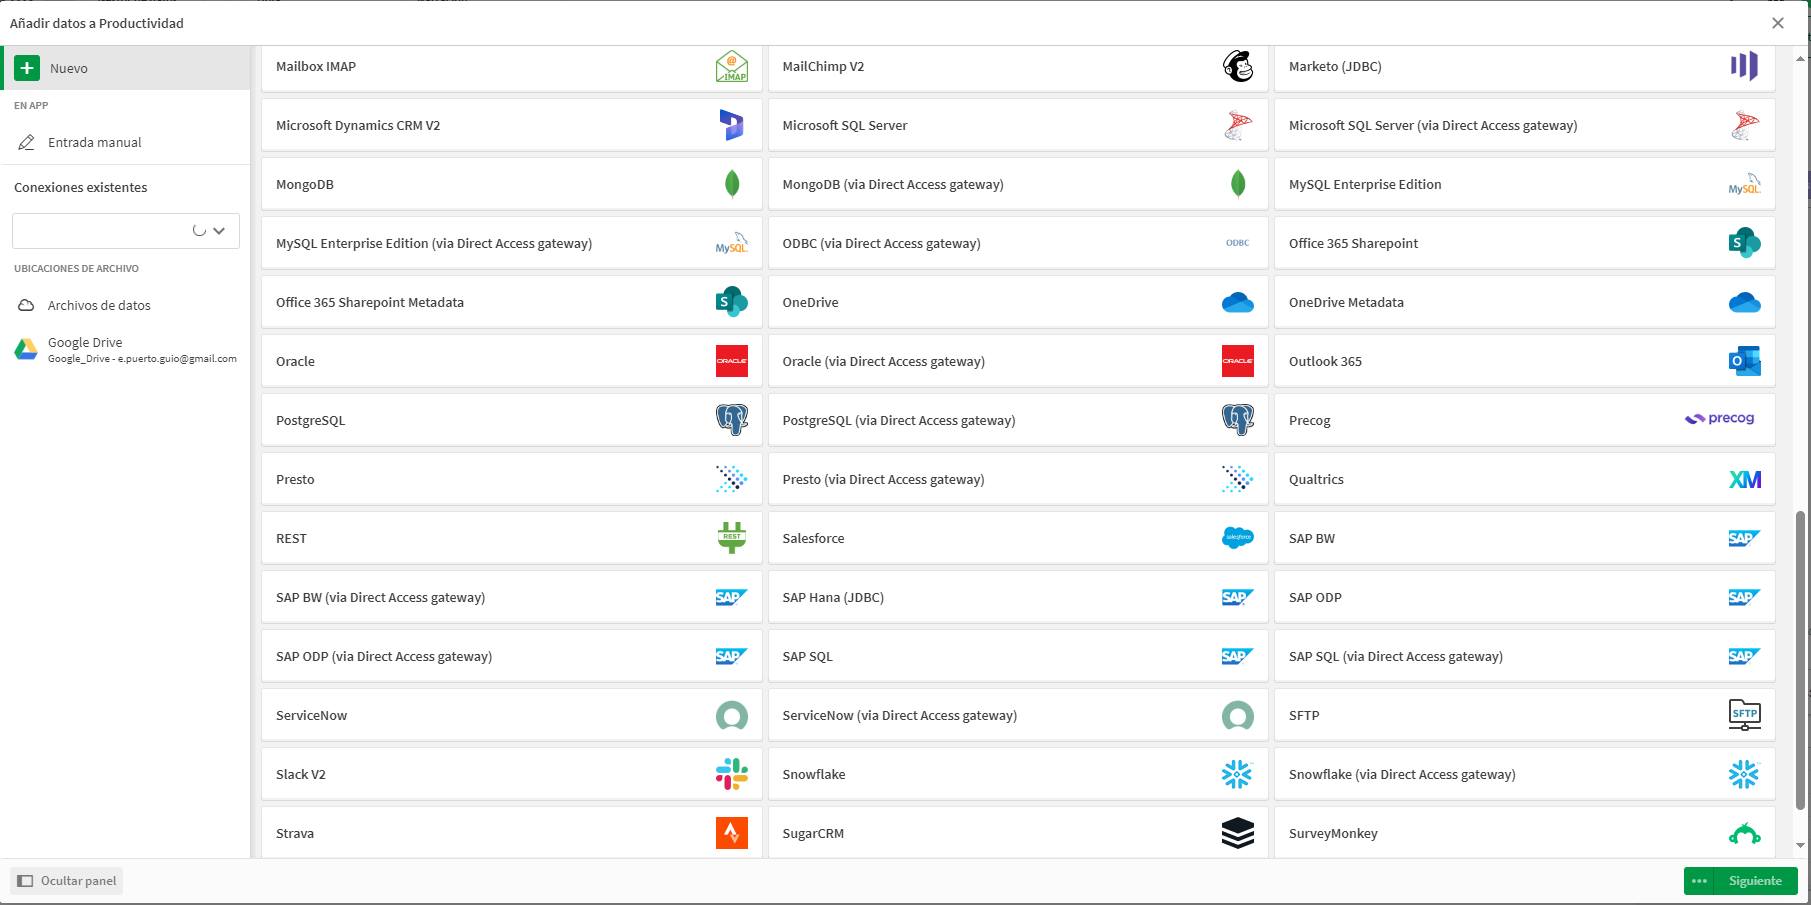
\includegraphics[width=4.53in]{media 2/image7} 

}

\caption{Tipos de archivos que pueden cargarse a Qlik Cloud}\label{fig:unnamed-chunk-11}
\end{figure}

\hypertarget{caso-pruxe1ctico-uso-de-looker-studio-en-el-sector-petrolero}{%
\paragraph{Caso Práctico: Uso de Looker Studio en el Sector Petrolero}\label{caso-pruxe1ctico-uso-de-looker-studio-en-el-sector-petrolero}}

Durante el caso práctico, Looker Studio demostró su capacidad para integrarse eficazmente con diversas fuentes de datos, especialmente a través de Google Drive y otros servicios de Google.
Esta versatilidad permite a la empresa adaptarse rápidamente a cambios en sus sistemas de información, mejorando la eficiencia operativa y la toma de decisiones.

\hypertarget{conectividad-y-fuentes-de-datos-en-looker-studio}{%
\paragraph{Conectividad y Fuentes de Datos en Looker Studio}\label{conectividad-y-fuentes-de-datos-en-looker-studio}}

Looker Studio permite conectarse a una amplia variedad de fuentes de datos a través de conectores.
La conectividad incluye:

\begin{itemize}
\item
  Conectores Propios: Looker Studio ofrece conectores propios para sus productos principales, facilitando la integración con otros servicios de Google.
\item
  Conectores Asociados: Además de los conectores propios, Looker Studio maneja conectores asociados que son desarrollados por terceros y suelen ser de pago.
  Estos conectores permiten la conexión a datos derivados de software específicos.
\item
  Autenticación de Cuenta: Al usar un conector, primero se debe autenticar la cuenta desde el conector de esa aplicación.
  Por ejemplo, para vincular un archivo desde Google Drive, primero se debe registrar la cuenta de Google Drive para que Looker Studio pueda enlazar y conectar a los datos.
\end{itemize}

\begin{figure}

{\centering 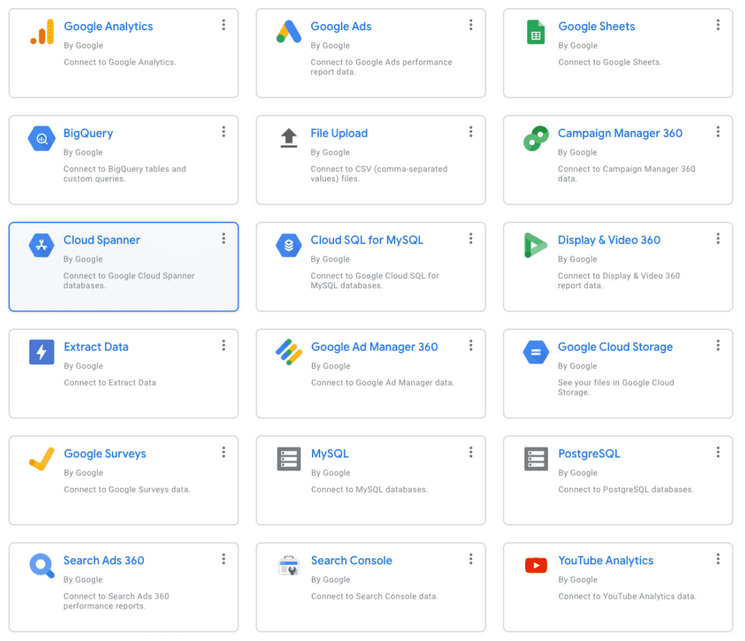
\includegraphics[width=3.72in]{media 2/image8} 

}

\caption{Tipos de archivos que pueden cargarse a Looker Studio}\label{fig:unnamed-chunk-12}
\end{figure}

La información anterior puede ser resumida en la tabla siguiente:

\begin{table}[H]

\caption{\label{tab:unnamed-chunk-13}Comparación de Herramientas de Visualización de Datos en el Sector Petrolero}
\centering
\fontsize{9}{11}\selectfont
\begin{tabular}[t]{>{\raggedright\arraybackslash}p{10em}|>{\raggedright\arraybackslash}p{15em}|>{\raggedright\arraybackslash}p{10em}}
\hline
Herramienta & Fuentes.de.Datos.Soportadas & Integración\\
\hline
Power BI Desktop & Bases de datos, servicios en la nube, archivos planos & Eficaz con otros softwares de Microsoft como SharePoint y Office\\
\hline
Qlik Cloud & Aplicaciones SaaS, bases de datos, almacenes de datos en la nube, SAP HANA & Conexión directa con SAP HANA, crucial para la gestión de mantenimiento con SAP\\
\hline
Looker Studio & Conectores propios para productos de Google, conectores asociados de terceros & Eficaz con Google Drive y otros servicios de Google\\
\hline
\end{tabular}
\end{table}

\hypertarget{capacidades-de-transformaciuxf3n-de-datos}{%
\subsubsection{Capacidades de Transformación de Datos}\label{capacidades-de-transformaciuxf3n-de-datos}}

\hypertarget{tipos-de-transformaciones}{%
\paragraph{Tipos de Transformaciones}\label{tipos-de-transformaciones}}

\textbf{Pregunta:} ¿Qué tipo de operaciones de transformación de datos soporta cada herramienta (filtrado, agregación, pivot, uniones, etc.)?

\hypertarget{facilidad-de-uso}{%
\paragraph{Facilidad de Uso}\label{facilidad-de-uso}}

\textbf{Pregunta:} ¿Qué tan intuitivas y fáciles de usar son las interfaces para transformar datos?

Se miden tres aspectos fundamentales:

\begin{enumerate}
\def\labelenumi{\arabic{enumi}.}
\item
  \textbf{Capacidad para Arrastrar y Soltar:}

  \begin{itemize}
  \tightlist
  \item
    Capacidad para mover columnas y elementos gráficos usando el ratón, lo que facilita la manipulación de los datos.
  \end{itemize}
\item
  \textbf{Previsualización de Datos:}

  \begin{itemize}
  \tightlist
  \item
    Posibilidad de tener una vista previa de los datos en tiempo real para ver las afectaciones de acuerdo con las acciones que se apliquen.
  \end{itemize}
\item
  \textbf{Menús Contextuales:}

  \begin{itemize}
  \tightlist
  \item
    Menús de apoyo con información relevante al dar clic derecho sobre un elemento.
  \end{itemize}
\end{enumerate}

\hypertarget{capacidades-etl-extract-transform-load}{%
\paragraph{Capacidades ETL (Extract, Transform, Load)}\label{capacidades-etl-extract-transform-load}}

\textbf{Pregunta:} ¿Proporciona funcionalidades completas de ETL o requiere herramientas adicionales?

\hypertarget{power-bi}{%
\subparagraph{Power Bi}\label{power-bi}}

Cuenta con un módulo robusto para la transformación de datos, permite la identificación de valore nulos en los campos, así como el tratamiento que se les da a estos, remplazarlos, eliminarlos o mantenerlos si es el caso, permite mediante el arrastre con el mouse mover las columnas, maneja menús emergentes de apoyo dando clik con el botón derecho del mouse sobre los campos, permite tener una visualización de los datos con las transformaciones y ajustes realizados.

\begin{figure}

{\centering 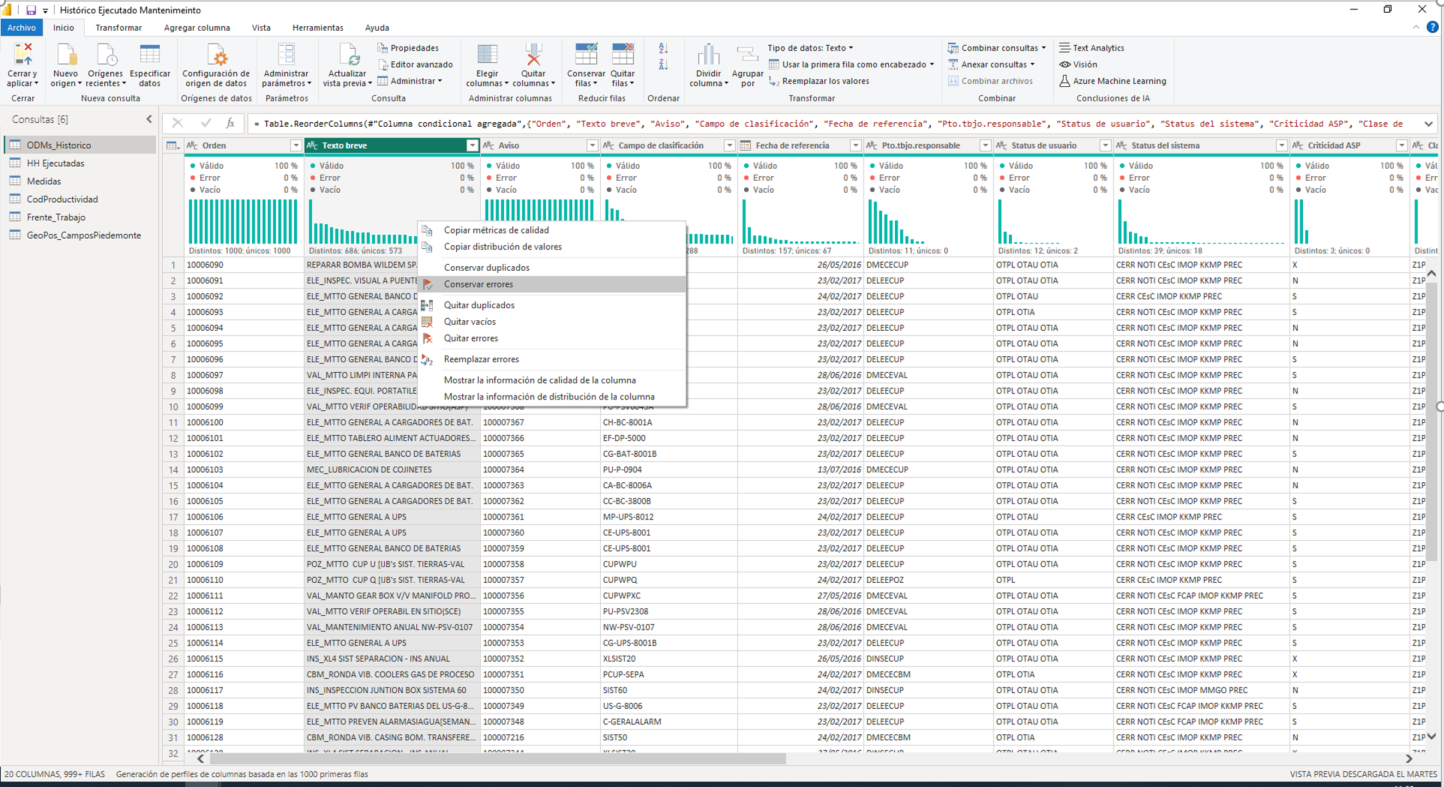
\includegraphics[width=5.78in]{media 2/image9} 

}

\caption{Transformaciones con Power Bi}\label{fig:unnamed-chunk-14}
\end{figure}

Mediante DAX y Lenguaje M se puede personalizar Consultas y generar medidas de acuerdo a las necesidades que requiera la visualización.
Para este caso se crearon columnas calculadas, medidas requeridas para el proceso de visualización de los datos, descritos en la fase de comprensión de los datos.
Este proceso fue relativamente fácil de implementar, no requiere un nivel avanzado en programación, se encuentra buen material de apoyo.

La interface que ofrece power BI es muy amigable e intuitiva, permite la organización de los datos visualmente en tablas que se pueden relacionar con acciones sencillas como clic y arrastre.
En power BI las acciones de transformación que se realizan sobre los datos quedan programadas para que se apliquen a nuevos datos que ingresen tras la actualización de las tablas.

\begin{figure}

{\centering 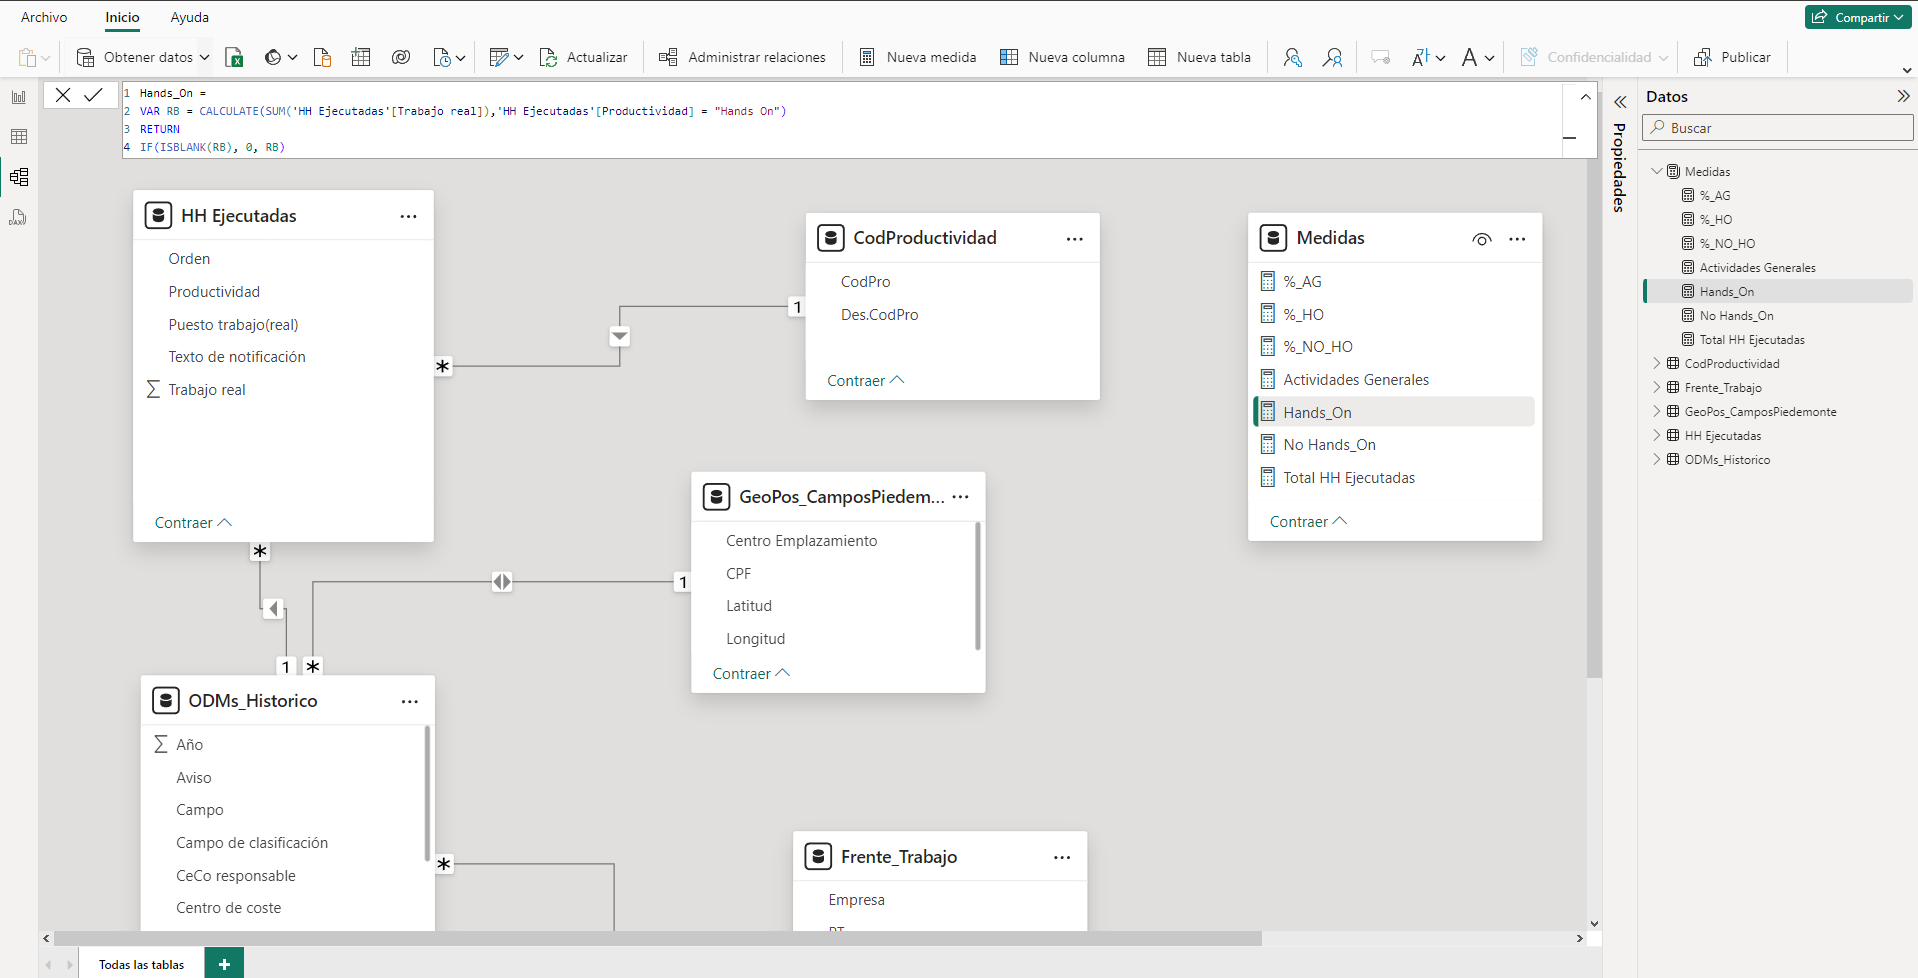
\includegraphics[width=4.8in]{media 2/image10} 

}

\caption{Transformaciones con Power Bi}\label{fig:unnamed-chunk-15}
\end{figure}

\hypertarget{qlik-cloud}{%
\subparagraph{Qlik Cloud}\label{qlik-cloud}}

Cuenta con un módulo robusto para la transformación de datos, permite la identificación de valore nulos en los campos, así como el tratamiento que se les da a estos, remplazarlos, eliminarlos o mantenerlos si es el caso, no permite mediante el arrastre con el mouse mover las columnas, maneja menús emergentes de apoyo dando clik con mouse sobre los campos, permite tener una visualización de los datos con las transformaciones y ajustes realizados.

\begin{figure}

{\centering 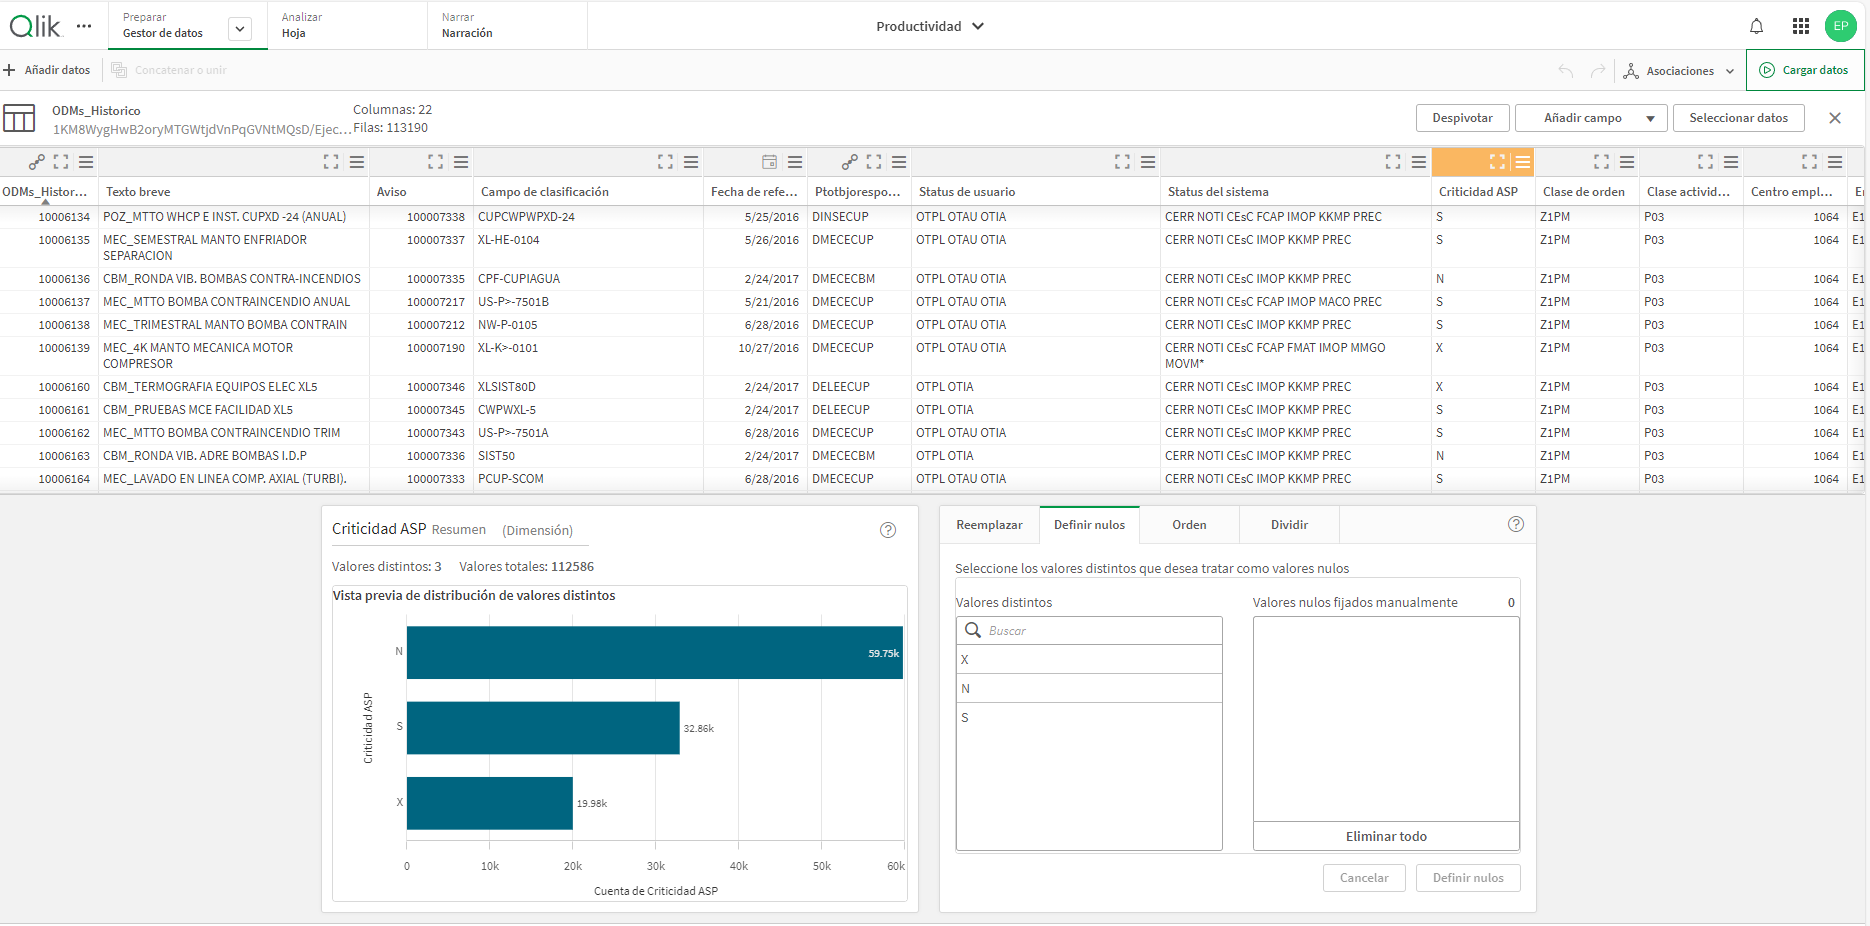
\includegraphics[width=4.68in]{media 2/image11} 

}

\caption{Transformaciones con Qlik Cloud}\label{fig:unnamed-chunk-16}
\end{figure}

La generación de medidas es robusta, cuenta con funciones predefinidas, sencillas de aplicar en las visualizaciones según se requiera.
Para el caso práctico se implementaron los requerimientos de algoritmos planteados en la fase de comprensión de los daros.

\begin{figure}

{\centering 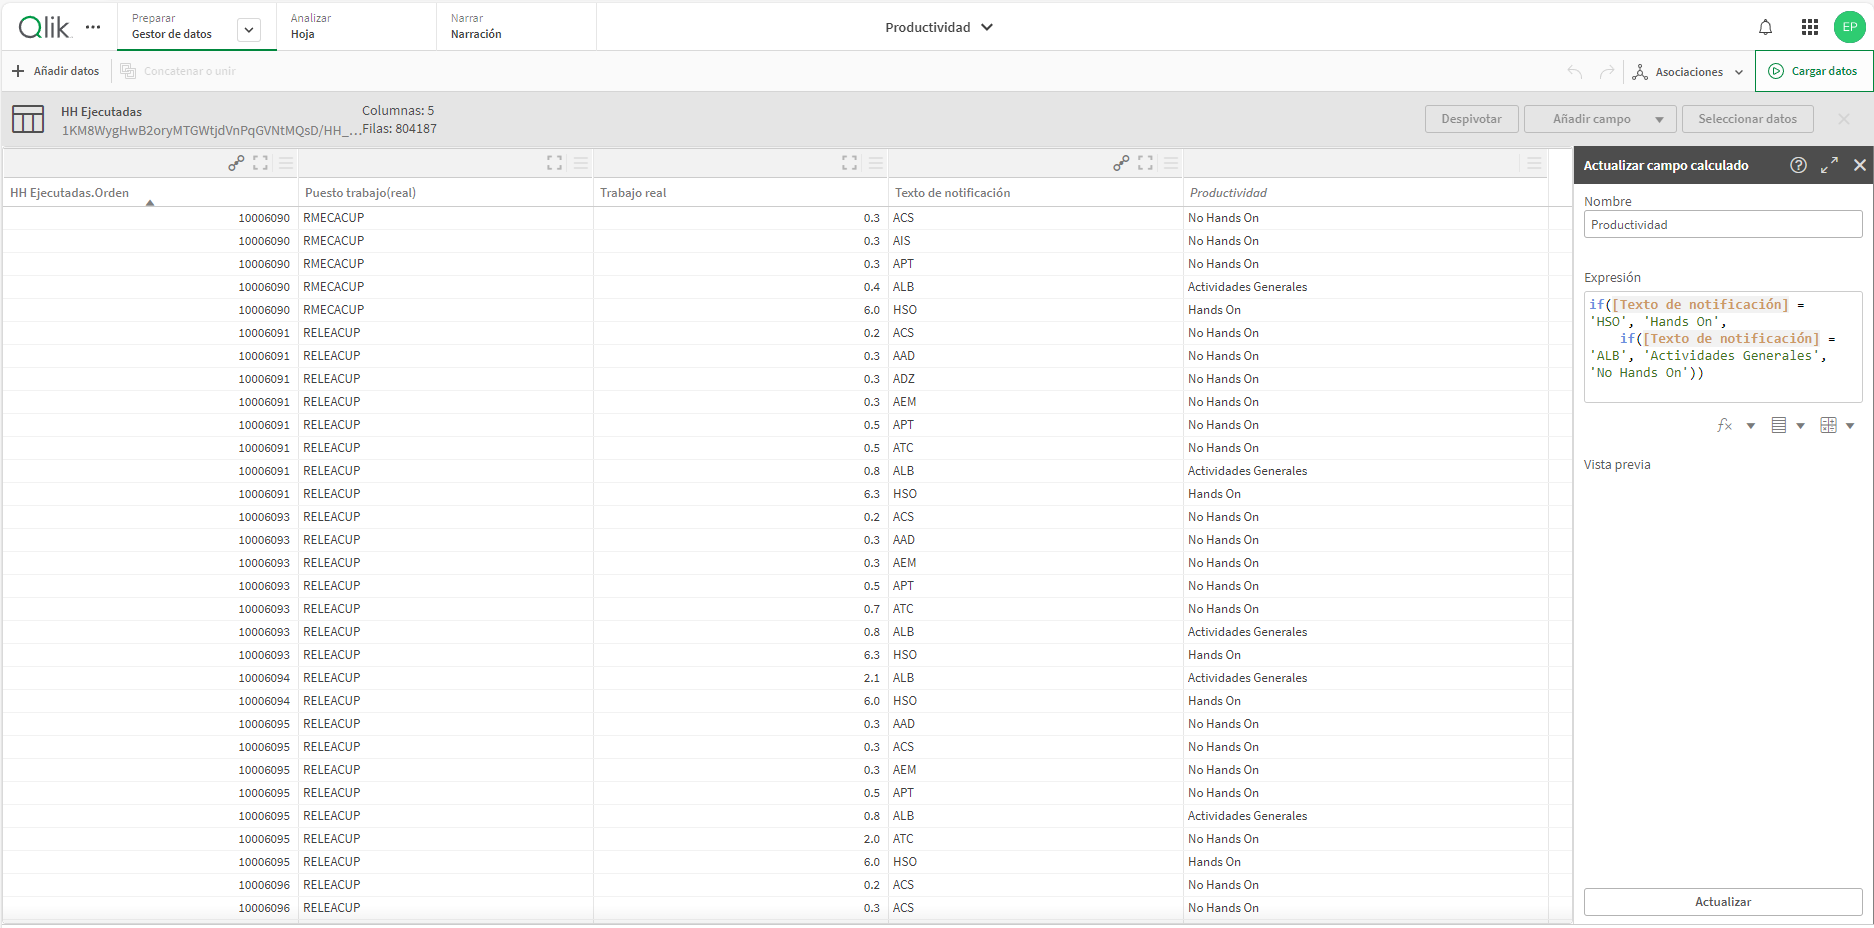
\includegraphics[width=4.68in]{media 2/image12} 

}

\caption{Transformado datos con Qlik Cloud}\label{fig:unnamed-chunk-17}
\end{figure}

\hypertarget{looker-studio}{%
\subparagraph{Looker Studio}\label{looker-studio}}

No cuenta con un módulo robusto como el caso de Power BI y Qlik, sin embargo, se pueden hacer transformaciones básicas, no permite tener una visualización de los datos.
Se debe complementar con Google Sheets o BigQuery para realizar tareas de transformación avanzadas.

\begin{figure}

{\centering 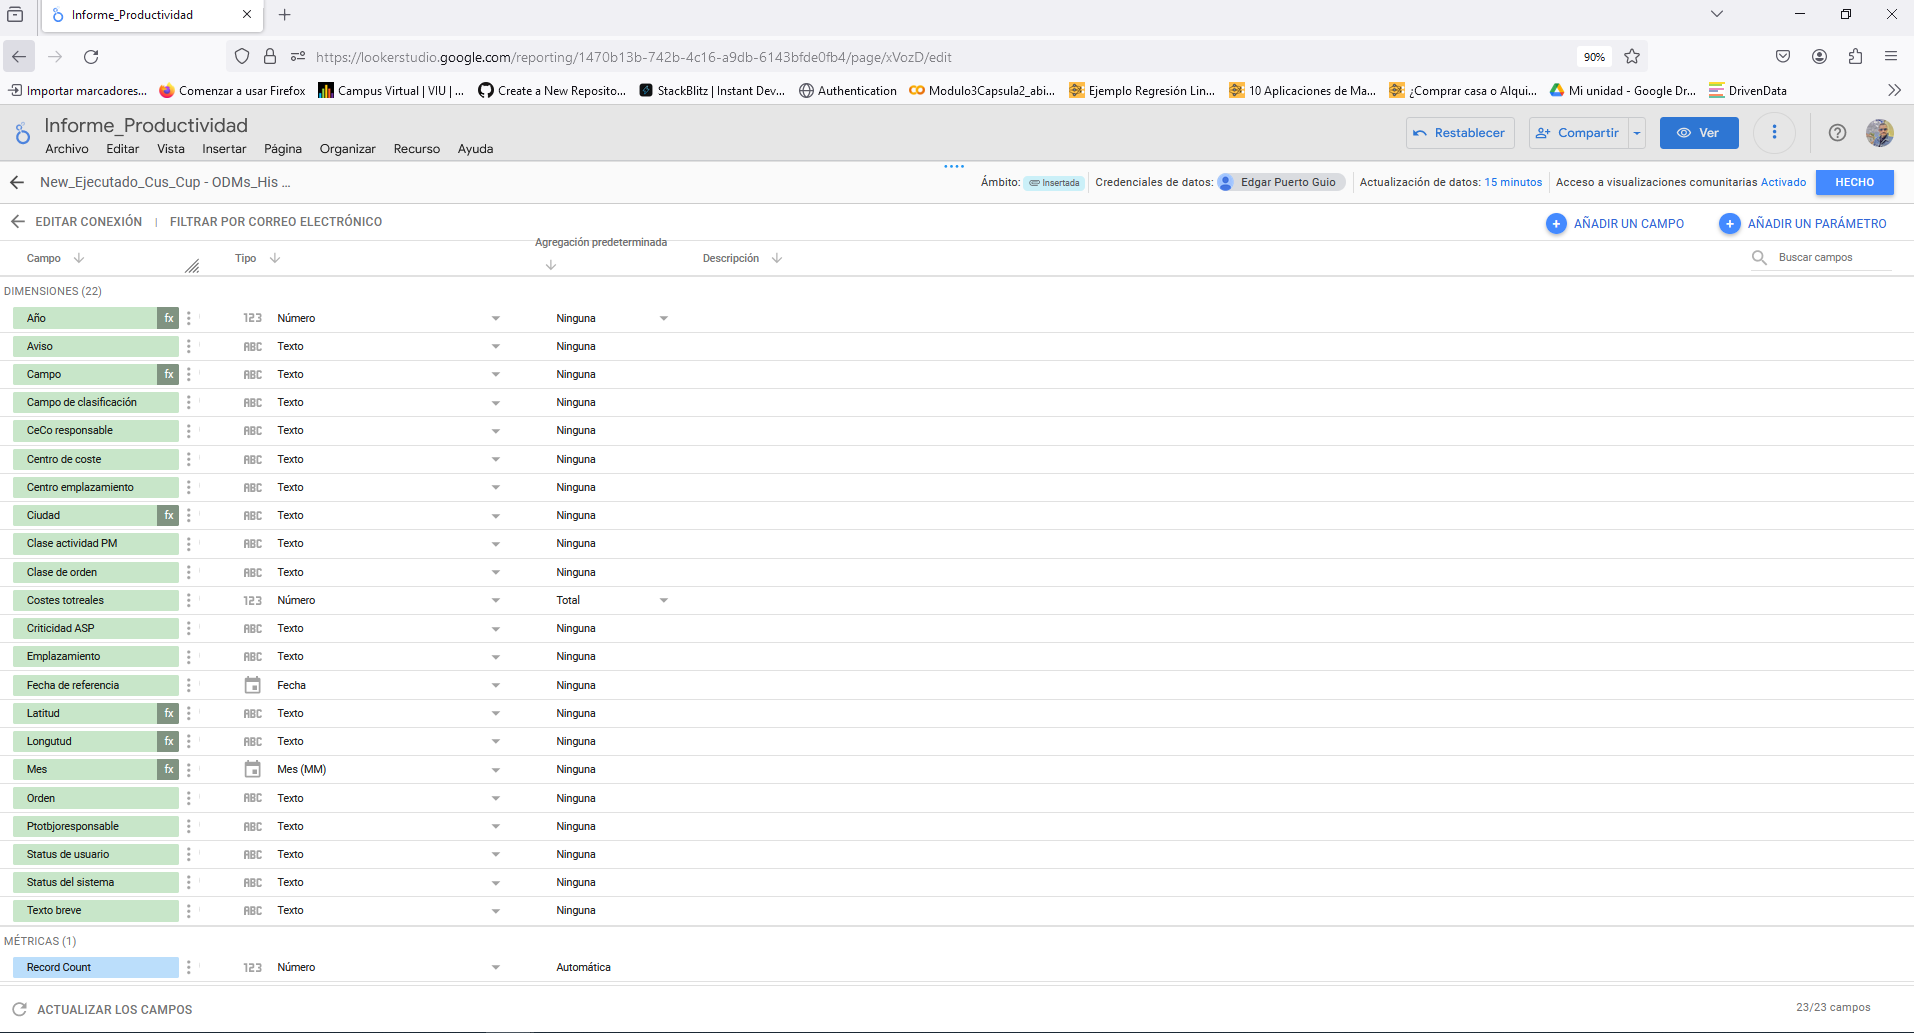
\includegraphics[width=4.78in]{media 2/image13} 

}

\caption{Transformación de datos con Looker Studio}\label{fig:unnamed-chunk-18}
\end{figure}

\newpage

\hypertarget{seguridad}{%
\subsubsection{Seguridad}\label{seguridad}}

La seguridad es un aspecto crítico en las herramientas de visualización de datos, especialmente cuando se manejan datos sensibles y confidenciales.

\hypertarget{power-bi-1}{%
\paragraph{Power BI}\label{power-bi-1}}

Se implementa seguridad mediante Seguridad la creación de roles y permisos de visualización de datos dependiendo el rol.

\begin{figure}

{\centering 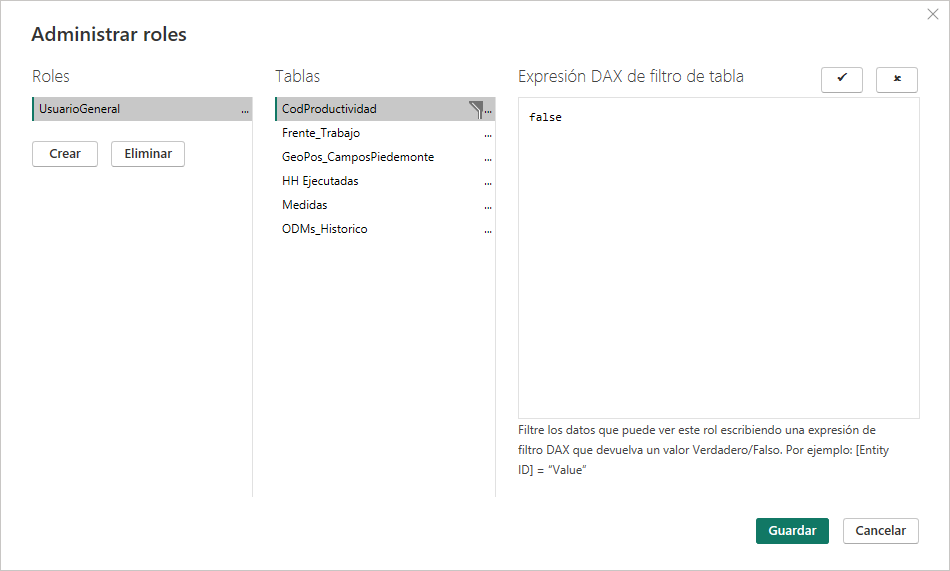
\includegraphics[width=3.8in]{media 2/image14} 

}

\caption{Seguridad en Power Bi}\label{fig:unnamed-chunk-19}
\end{figure}

\hypertarget{autenticaciuxf3n-y-autorizaciuxf3n}{%
\subparagraph{Autenticación y Autorización:}\label{autenticaciuxf3n-y-autorizaciuxf3n}}

\begin{itemize}
\item
  \textbf{Azure Active Directory (AAD):} Power BI utiliza Azure Active Directory para la autenticación y autorización de usuarios, ofreciendo características avanzadas como Multi-Factor Authentication (MFA) y Single Sign-On (SSO).
\item
  \textbf{Roles y Permisos:} Permite definir roles y permisos específicos para controlar el acceso a los datos y las funcionalidades de Power BI. Los administradores pueden otorgar permisos de lectura, escritura y administración según sea necesario.
\end{itemize}

\hypertarget{seguridad-de-los-datos}{%
\subparagraph{Seguridad de los Datos:}\label{seguridad-de-los-datos}}

\begin{itemize}
\item
  \textbf{Encriptación:} Power BI cifra los datos tanto en tránsito como en reposo utilizando tecnologías estándar de la industria.
\item
  \textbf{Row-Level Security (RLS):} Permite aplicar reglas de seguridad a nivel de fila para garantizar que los usuarios solo puedan ver los datos que les están autorizados.
\end{itemize}

\hypertarget{conformidad-y-certificaciones}{%
\subparagraph{Conformidad y Certificaciones:}\label{conformidad-y-certificaciones}}

\begin{itemize}
\tightlist
\item
  \textbf{Cumplimiento Normativo:} Power BI cumple con varias normativas de seguridad y privacidad, incluyendo GDPR, HIPAA y SOC.
\end{itemize}

\hypertarget{looker}{%
\paragraph{Looker}\label{looker}}

Filtrado por dirección de correo electrónico para asegurar los datos a nivel de fila, los informes solicitan permiso para acceder a la dirección de correo electrónico del lector con el objetivo de parametrizar los datos que se visualizan. Cuando los usuarios dan su consentimiento para compartir su dirección de correo con ese informe, la fuente de datos subyacente puede usarla para devolver solo los datos asociados a esa dirección de correo. Esto se conoce como ``seguridad de los datos a nivel de fila''.

\begin{figure}

{\centering 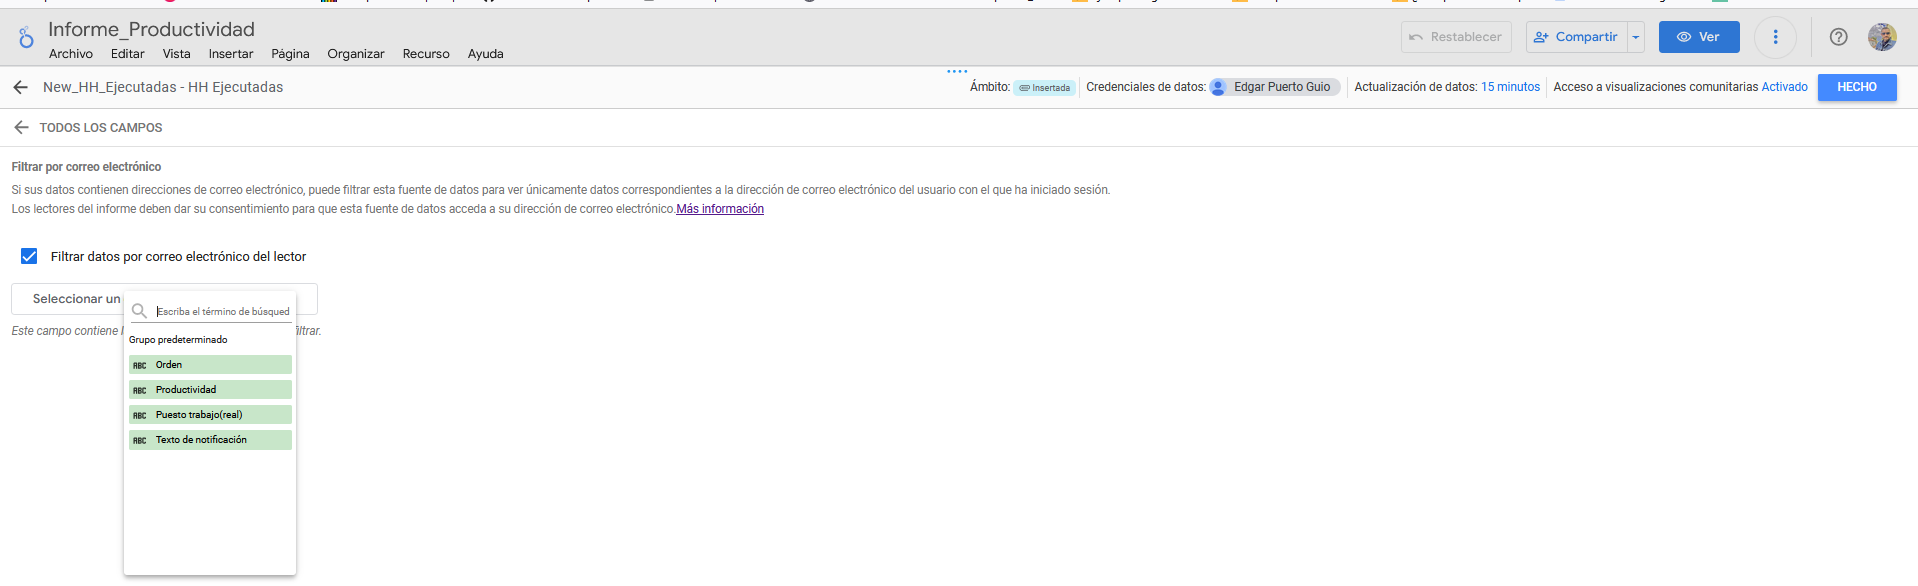
\includegraphics[width=4.8in]{media 2/image16} 

}

\caption{Seguridad en Looker Studio}\label{fig:unnamed-chunk-20}
\end{figure}

\hypertarget{autenticaciuxf3n-y-autorizaciuxf3n-1}{%
\subparagraph{Autenticación y Autorización:}\label{autenticaciuxf3n-y-autorizaciuxf3n-1}}

\begin{itemize}
\item
  \textbf{Integraciones SSO:} Looker soporta integraciones con múltiples proveedores de SSO, incluyendo SAML, LDAP y OAuth.
\item
  \textbf{Control de Acceso Granular:} Looker permite definir permisos detallados a nivel de usuario, grupo y rol, controlando el acceso a datos y funcionalidades específicas.
\end{itemize}

\hypertarget{seguridad-de-los-datos-1}{%
\subparagraph{Seguridad de los Datos:}\label{seguridad-de-los-datos-1}}

\begin{itemize}
\item
  \textbf{Encriptación:} Los datos en Looker están encriptados tanto en tránsito como en reposo.
  Utiliza HTTPS para las comunicaciones y encriptación en reposo para los datos almacenados.
\item
  \textbf{Data Modeling Layer:} Looker utiliza una capa de modelado de datos centralizada que permite controlar y auditar el acceso a los datos de manera eficiente.
\end{itemize}

\hypertarget{conformidad-y-certificaciones-1}{%
\subparagraph{Conformidad y Certificaciones:}\label{conformidad-y-certificaciones-1}}

\begin{itemize}
\tightlist
\item
  \textbf{Cumplimiento Normativo:} Looker cumple con normativas de seguridad como SOC 2, ISO 27001 y GDPR.
\end{itemize}

\hypertarget{qlik-cloud-1}{%
\paragraph{Qlik Cloud}\label{qlik-cloud-1}}

Ofrece un robusto conjunto de herramientas para asegurar que la empresa mantenga la protección de los datos bajo las regulaciones pertinentes. La autenticación y autorización junto con la encriptación y seguridad a nivel de filas garantiza que únicamente los usuarios autorizados tengan acceso a la información pertinente.

\begin{figure}

{\centering 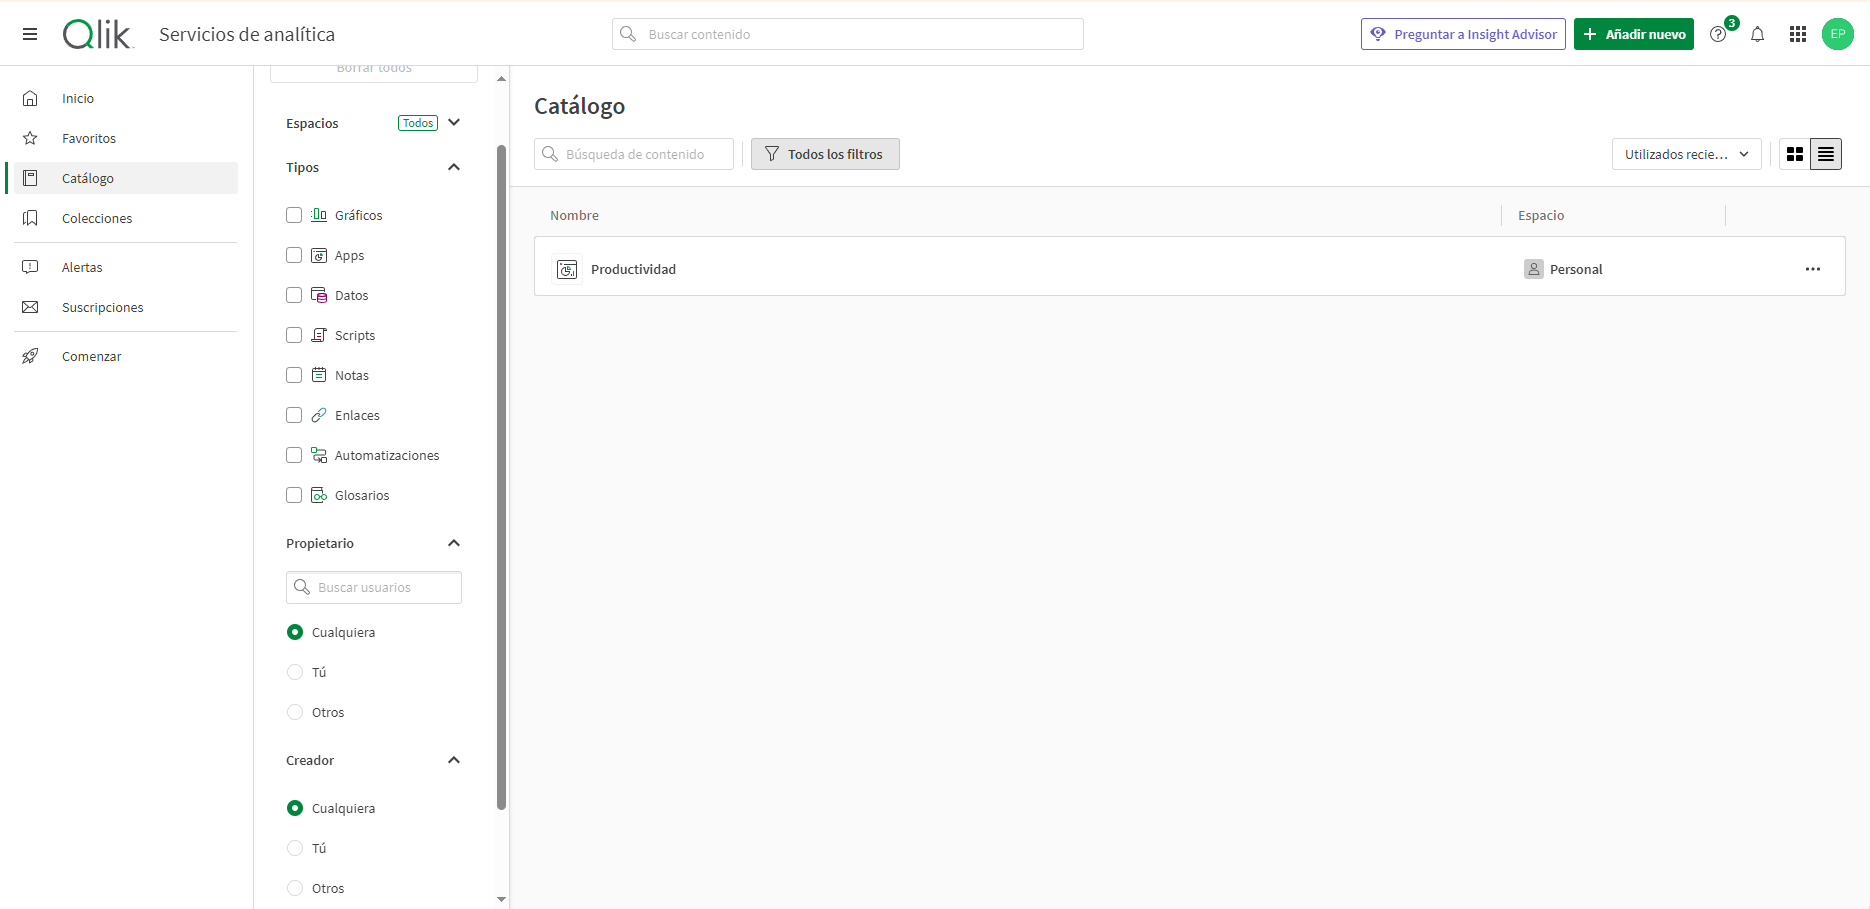
\includegraphics[width=4.68in]{media 2/image15} 

}

\caption{Seguridad en Qlik Cloud}\label{fig:unnamed-chunk-21}
\end{figure}

\hypertarget{autenticaciuxf3n-y-autorizaciuxf3n-2}{%
\subparagraph{Autenticación y Autorización:}\label{autenticaciuxf3n-y-autorizaciuxf3n-2}}

\begin{itemize}
\item
  \textbf{Qlik Account y SSO:} Qlik Cloud utiliza Qlik Account para la autenticación, con soporte para SSO a través de SAML y OpenID Connect.
\item
  \textbf{Roles y Permisos:} Qlik Cloud permite la configuración de roles y permisos específicos para gestionar el acceso a aplicaciones, datos y funcionalidades.
\end{itemize}

\hypertarget{seguridad-de-los-datos-2}{%
\subparagraph{Seguridad de los Datos:}\label{seguridad-de-los-datos-2}}

\begin{itemize}
\item
  \textbf{Encriptación:} Qlik Cloud encripta los datos en tránsito utilizando HTTPS y en reposo utilizando encriptación de disco.
\item
  \textbf{Section Access:} Qlik Cloud ofrece control de acceso a nivel de documento y campo mediante la funcionalidad de Section Access, que permite definir reglas de acceso específicas para usuarios y grupos.
\end{itemize}

\hypertarget{conformidad-y-certificaciones-2}{%
\subparagraph{Conformidad y Certificaciones:}\label{conformidad-y-certificaciones-2}}

\begin{itemize}
\tightlist
\item
  \textbf{Cumplimiento Normativo:} Qlik Cloud cumple con normativas de seguridad y privacidad como GDPR y SOC 2.
\end{itemize}

\begin{table}[H]

\caption{\label{tab:unnamed-chunk-22}Comparación de Seguridad}
\centering
\fontsize{9}{11}\selectfont
\begin{tabular}[t]{>{\raggedright\arraybackslash}p{10em}|>{\raggedright\arraybackslash}p{20em}|>{\raggedright\arraybackslash}p{20em}|>{}p{15em}}
\hline
Herramienta & Fuentes.de.Datos.Soportadas & Integración\\
\hline
Power BI Desktop & Bases de datos, servicios en la nube, archivos planos & Eficaz con otros softwares de Microsoft como SharePoint y Office\\
\hline
Qlik Cloud & Aplicaciones SaaS, bases de datos, almacenes de datos en la nube, SAP HANA & Conexión directa con SAP HANA, crucial para la gestión de mantenimiento con SAP\\
\hline
Looker Studio & Conectores propios para productos de Google, conectores asociados de terceros & Eficaz con Google Drive y otros servicios de Google\\
\hline
\end{tabular}
\end{table}

\hypertarget{geolocalizaciuxf3n}{%
\subsubsection{Geolocalización}\label{geolocalizaciuxf3n}}

Para el caso práctico se estructura tabla con información del Campo petrolero y la georreferenciación que se utilizara en Power BI, Qlik Cloud y Loker Studio

\begin{table}[H]

\caption{\label{tab:unnamed-chunk-23}Datos de geolocalización}
\centering
\fontsize{9}{11}\selectfont
\begin{tabular}[t]{l|l|l|l|l}
\hline
CPF & Centro.Emplazamiento & Ciudad & Latitud & Longitud\\
\hline
Cusiana & 1063 & Tauramena & 5.0009 & -72.7062\\
\hline
Cupiagua & 1064 & Aguazul & 5.2099 & -72.60\\
\hline
floreña & 1061 & Yopal & 5.3476 & -72.3958\\
\hline
\end{tabular}
\end{table}

\hypertarget{power-bi-2}{%
\paragraph{Power BI}\label{power-bi-2}}

Fácil implementación requiere estructuración previa de Latitudes y Longitudes asociadas a los CPF o centros de acopio petroleros, en el control de mapa se asocia los campos Latitud y longitud, en el control casilla ``Información sobre herramienta'' se pueden adicionar los campos que se requieran mostrar como información adicional al seleccionar la burbuja del punto de georreferenciado. Para el caso práctico se realiza ejercicio con Mapa básico y Mapa ArcGIS.

\begin{figure}

{\centering 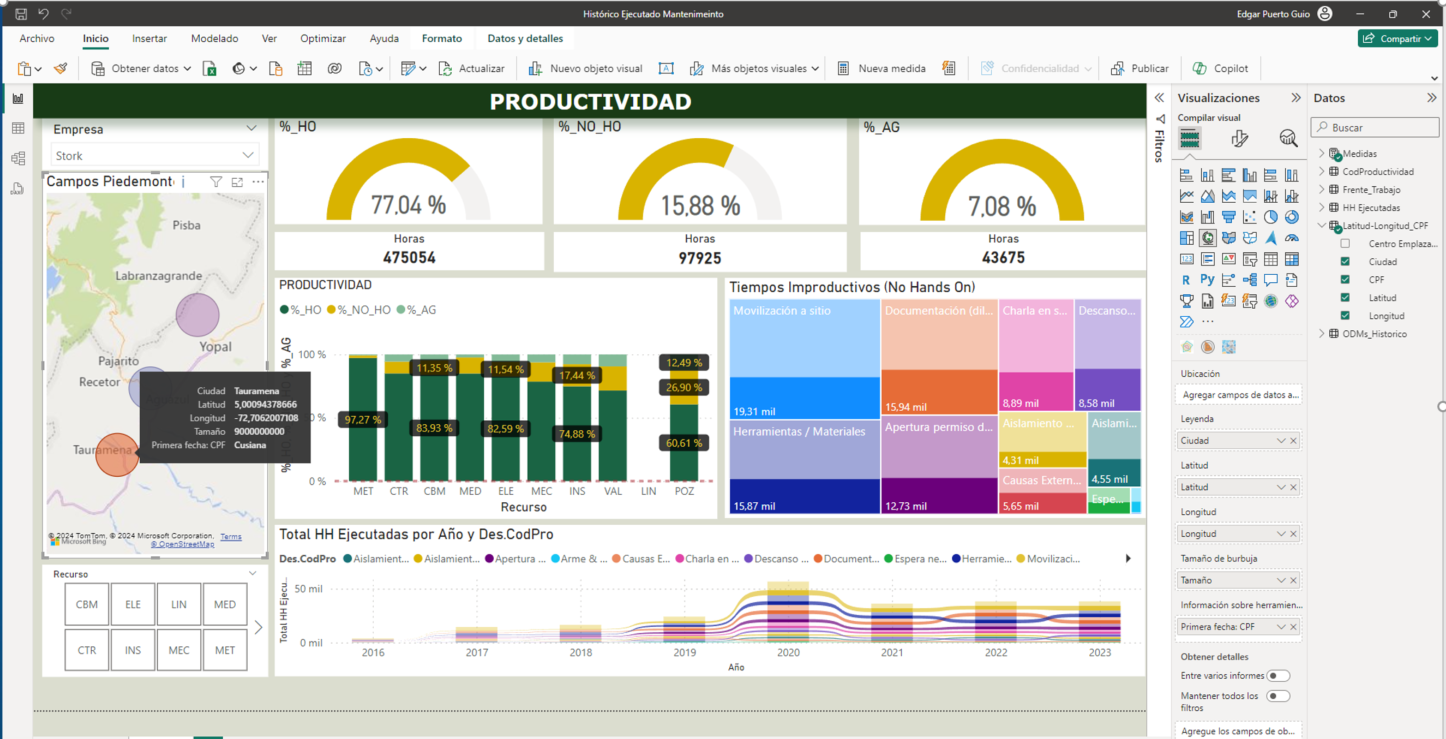
\includegraphics[width=5.78in]{media 2/image18} 

}

\caption{Dashboard geolocalización con Power Bi}\label{fig:unnamed-chunk-24}
\end{figure}

\hypertarget{qlik-cloud-2}{%
\paragraph{Qlik Cloud}\label{qlik-cloud-2}}

Fácil implementación, al igual que en power BI se debe estructura las latitudes y longitudes para los centros de acopio o CPF.

\begin{figure}

{\centering 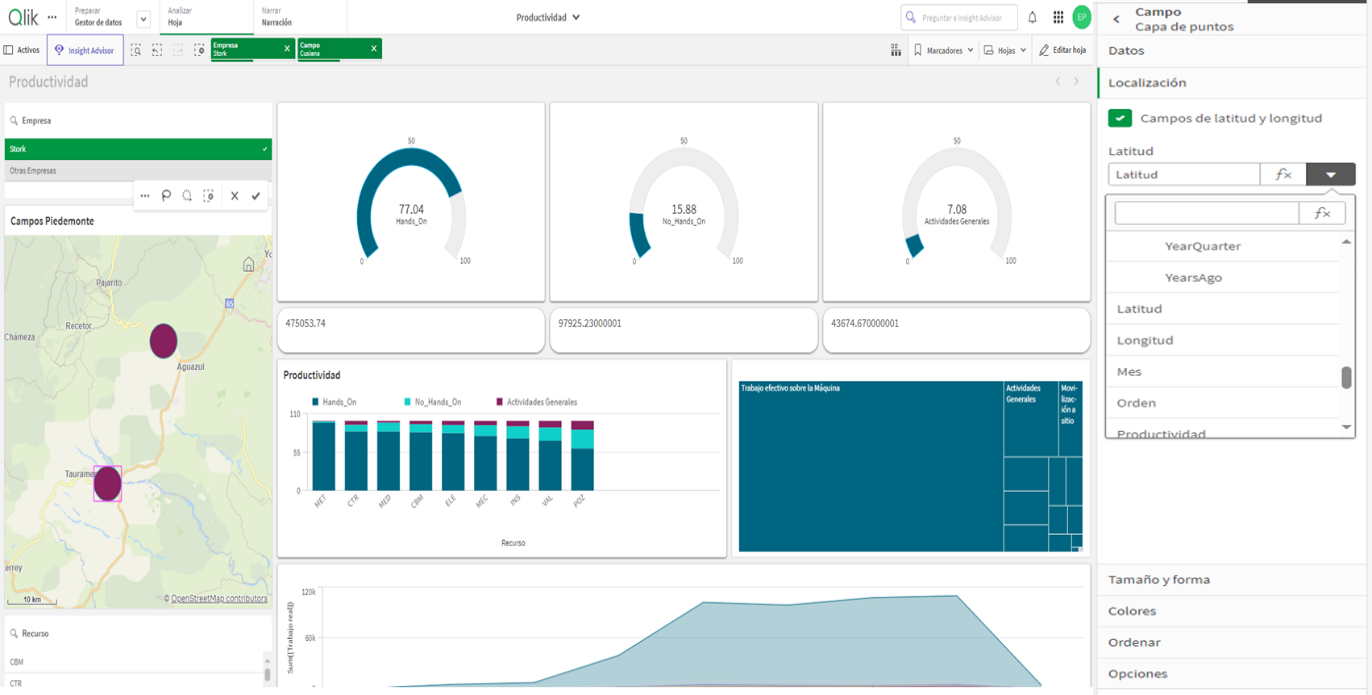
\includegraphics[width=5.49in]{media 2/image20} 

}

\caption{Dashboard geolocalización con Qlik Cloud}\label{fig:unnamed-chunk-25}
\end{figure}

\hypertarget{looker-studio-1}{%
\paragraph{Looker Studio}\label{looker-studio-1}}

Fácil implementación, la visualización de los centros de acopio se realiza asociando el campo ciudad en el área de ubicación del control de mapa.

\begin{figure}

{\centering 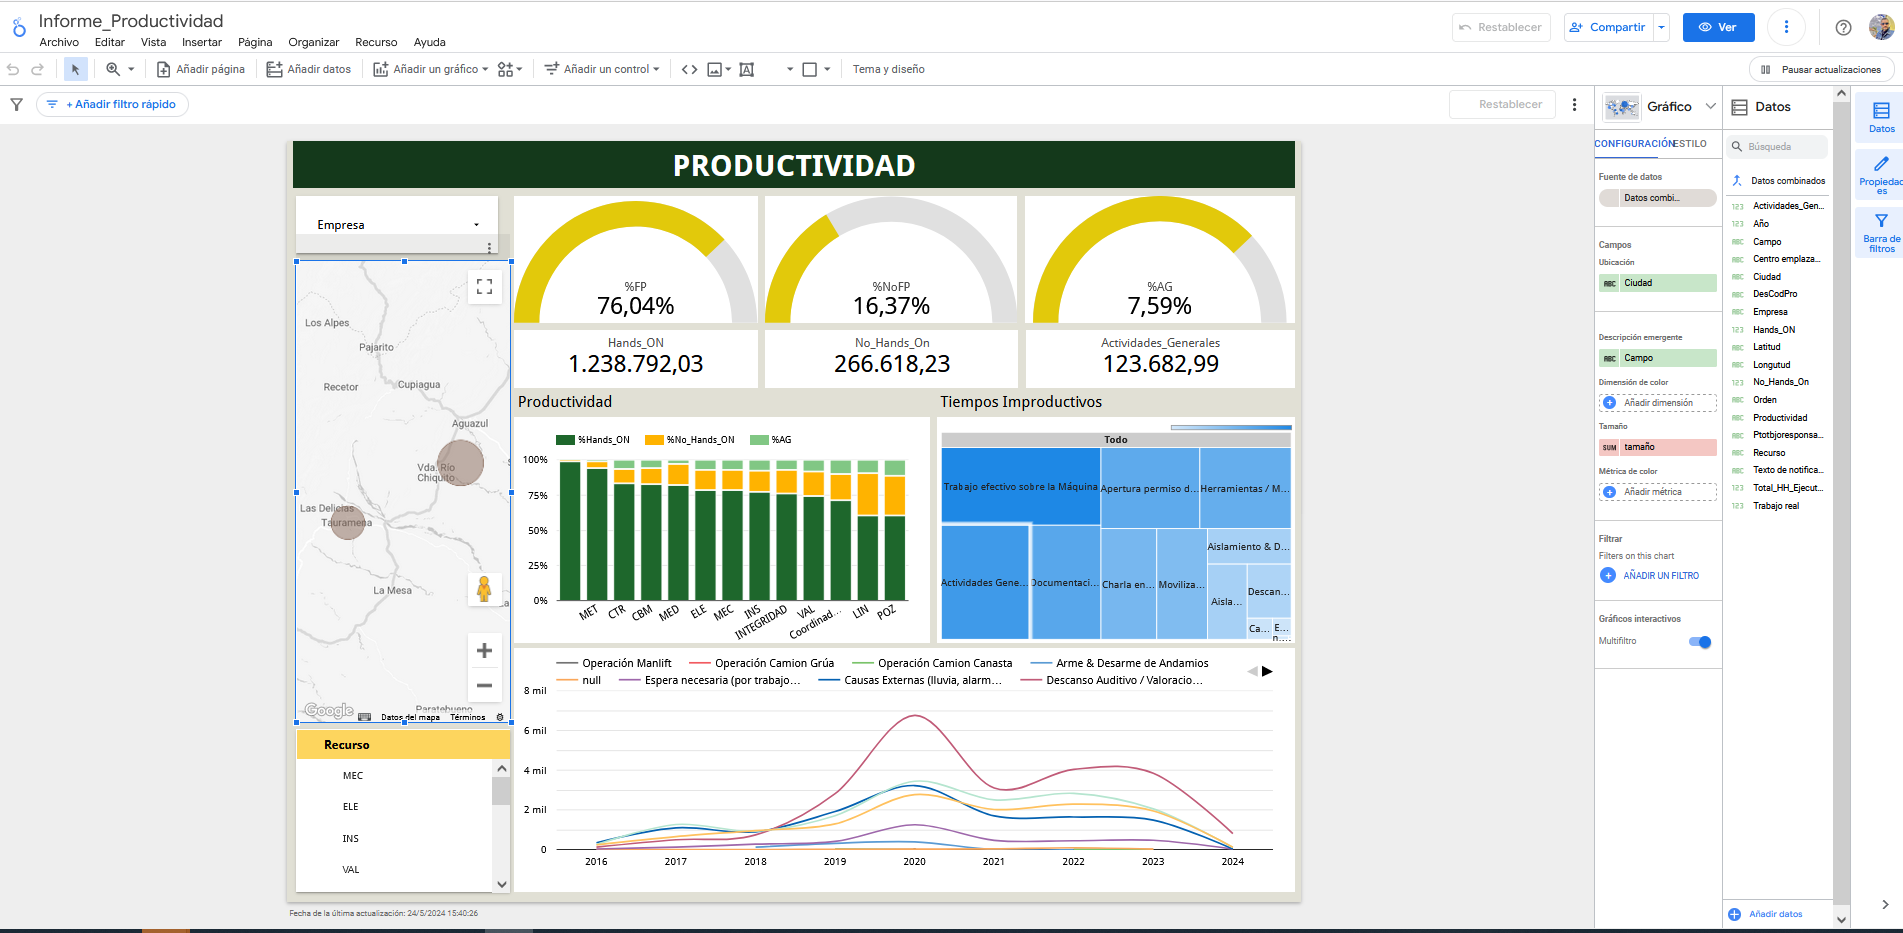
\includegraphics[width=4.76in]{media 2/image21} 

}

\caption{Dashboard geolocalización con Looker Studio}\label{fig:unnamed-chunk-26}
\end{figure}

\hypertarget{interfaz-de-usuario-y-experiencia-de-usuario}{%
\subsubsection{Interfaz de Usuario y Experiencia de Usuario}\label{interfaz-de-usuario-y-experiencia-de-usuario}}

\textbf{Power BI}

Es una herramienta fácil de aprender, muy intuitiva. Si se cuenta con experiencia en programación DAX y M se pueden obtener muy buenos resultados personalizando la interfaz de acuerdo a los requerimientos que se tengan.
Cuenta con Power Query que es una herramienta poderosa para la limpieza y transformación de datos.
Permite la creación de informes personalizados mediante la funcionalidad de arrastrar y soltar.
Los tiempos de respuesta en el diseño de las visualizaciones y la consulta son rápidos.
Se integra muy buen con otros productos Microsoft para el caso práctico se estableció conexiones con Share Point.

\textbf{Qlik Cloud}

Interfaz con un diseño intuitivo y limpio, diseño minimalista funcionalidades de arrastre y soltar, la visualización es interactiva y se puede personalizar de acuerdo a las necesidades que se tengan.
Data Load Editor herramienta potente para cargar y transformar datos.
Al igual que Power BI, Qlik permite crear visualizaciones haciendo uso de la funcionalidad Arrastrar y soltar.
Qlik Ofrece un mayor nivel de personalización esta característica es una ventaja para usuarios avanzados, pero requiere una mayor curva de aprendizaje.

\textbf{Looker Studio}

Fácil uso al igual que Power BI la funcionalidad de arrastrar y soltar es clave en la elaboración de visualizaciones cundo el usuario no tiene gran experiencia.
Facilita el trabajo y toma de decisiones en equipo gracias a su colaboración en tiempo real.

\hypertarget{rendimiento-y-escalabilidad}{%
\subsubsection{Rendimiento y Escalabilidad}\label{rendimiento-y-escalabilidad}}

\begin{itemize}
\item
  \textbf{Power BI}
  La tecnología de compresión y modelado en memoria ``VertiPaq engine'' optimiza el rendimiento de las consultas, los datos con más frecuencia de consulta son almacenados en cache mejorando la velocidad de consulta, esto se puede evidenciar en el caso práctico donde se tiene un buen rendimiento de consulta de los datos histórico de mantenimiento en la visualización que se implementó.
\item
  \textbf{Qlik Cloud}
  El motor asociativo que maneja Qlik Cloud permite la consulta de grandes volúmenes de datos en tiempo real, al igual que Power BI los datos se cargan en memoria lo que permite una consulta y recuperación muy rápida, las visualizaciones se actualizan de manera interactiva cundo el usuario hace una seleccione. Todo esto se evidencia en el caso práctico desarrollado, se tiene una buena velocidad de consulta, la interacción visual de los datos al aplicar filtros es inmediata.
\item
  \textbf{Loker Studio}
  Tiende a ser más lento con grandes volúmenes de datos ya qie Looker Studio consulta directamente las fuentes de datos en lugar de almacenarlas y procesarlas localmente, si bien se cuenta con datos actualizados impacta significativamente en la velocidad de procesamiento de la información, esto se evidencia en el caso práctico desarrollado, donde la consulta de los datos es demasiado lenta; en esta mediada en particular power BI y Qlik Cloud muestran un rendimiento superior.
\end{itemize}

\hypertarget{soporte-y-comunidad}{%
\subsubsection{Soporte y Comunidad}\label{soporte-y-comunidad}}

\begin{itemize}
\item
  Power BI
  Se encuentra documentación amplia y detallada como guías de usuario, tutoriales en sitios de Microsoft, documentación técnica, foros, video tutoriales, en general se encuentra muy buen soporte y con una comunidad amplia de apoyo.
\item
  Qlik Cloud
  Al igual que Power BI se cuenta con documentación amplia y detallada como guías de usuario, tutoriales en sitios oficiales de Qlik, documentación técnica, foros, video tutoriales, en general se encuentra muy buen soporte y con una comunidad amplia de apoyo.
\item
  Looker Studio
  Cuenta con documentación técnica en el sitio oficial de Google no es tan completa y detallada si se compara con Power BI y Qlik Cloud.
\end{itemize}

\hypertarget{coste-y-licenciamiento}{%
\subsubsection{Coste y Licenciamiento}\label{coste-y-licenciamiento}}

\textbf{Power BI}

\begin{itemize}
\item
  Power BI Free: Disponible de forma gratuita, permite a los usuarios individuales crear y compartir informes y dashboards. Limitado a capacidades básicas y almacenamiento reducido.
\item
  Power BI Pro: Cuesta aproximadamente \$9.99 USD por usuario por mes. Incluye capacidades completas de colaboración, uso compartido y publicación de informes.
\item
  Power BI Premium: Tiene un costo que comienza en \$20 USD por usuario por mes (Premium Per User) o una tarifa mensual basada en la capacidad (Premium Capacity), que comienza en \$4,995 USD por recurso de capacidad por mes. Ofrece capacidades avanzadas, mayor capacidad de almacenamiento y características exclusivas como IA y análisis de big data.
\end{itemize}

Las versiones no pagas ofrecen: creación y visualización de informes y dashboards, conexión a diversas fuentes de datos, almacenamiento limitado.

\textbf{Qlik Cloud}

\begin{itemize}
\item
  Qlik Sense Business (Free Trial): Ofrece una prueba gratuita de 30 días.
\item
  Qlik Sense Business: Cuesta aproximadamente \$30 USD por usuario por mes. Incluye todas las capacidades necesarias para la mayoría de las organizaciones pequeñas y medianas.
\item
  Qlik Sense Enterprise SaaS: Precio personalizado según las necesidades de la empresa. Incluye características avanzadas, mayor capacidad de almacenamiento y funcionalidades empresariales.
\end{itemize}

Las versiones no pagas ofrecen: Prueba gratuita de 30 días con acceso a todas las características de Qlik Sense Business, Capacidades completas durante el período de prueba.

\textbf{Looker Studio}

\begin{itemize}
\item
  Looker Studio (anteriormente Google Data Studio): Es gratuito y ofrece todas las funcionalidades sin costo alguno.
\item
  Looker (la plataforma completa de análisis de datos): Tiene un costo personalizado basado en el tamaño y necesidades de la empresa.
\end{itemize}

Las versiones no pagas ofrecen: Acceso completo a Looker Studio sin costo, Creación ilimitada de informes y dashboards, Conexión a diversas fuentes de datos incluidas Google Analytics, Google Sheets y BigQuery.

\newpage

\hypertarget{modelado-1}{%
\subsection{Modelado}\label{modelado-1}}

\hypertarget{matriz-de-comparaciuxf3n-por-pares-para-los-criterios}{%
\subsubsection{Matriz de Comparación por Pares para los Criterios}\label{matriz-de-comparaciuxf3n-por-pares-para-los-criterios}}

Para la estructuración de esta matriz se evaluarán los criterios usando la siguiente escala de importancia:

\begin{itemize}
\item
  1: Los criterios son igualmente importantes.
\item
  3: El criterio de la fila es moderadamente más importante que el criterio de la columna.
\item
  1/3: El criterio de la columna es moderadamente más importante que el criterio de la fila.
\item
  5: El criterio de la fila es fuertemente más importante que el criterio de la columna.
\item
  1/5: El criterio de la columna es fuertemente más importante que el criterio de la fila.
\item
  7: El criterio de la fila es muy fuertemente más importante que el criterio de la columna.
\item
  1/7: El criterio de la columna es muy fuertemente más importante que el criterio de la fila.
\end{itemize}

\begin{table}[!h]

\caption{\label{tab:unnamed-chunk-27}Matriz de Comparación por Pares para los Criterios}
\centering
\begin{tabular}[t]{lllllllll}
\toprule
\multicolumn{1}{c}{\rotatebox{90}{Aspecto}} & \multicolumn{1}{c}{\rotatebox{90}{Conectividad}} & \multicolumn{1}{c}{\rotatebox{90}{Transformación de Datos}} & \multicolumn{1}{c}{\rotatebox{90}{Seguridad}} & \multicolumn{1}{c}{\rotatebox{90}{Geolocalización}} & \multicolumn{1}{c}{\rotatebox{90}{Interfaz de Usuario}} & \multicolumn{1}{c}{\rotatebox{90}{Rendimiento y Escalabilidad}} & \multicolumn{1}{c}{\rotatebox{90}{Soporte y Comunidad}} & \multicolumn{1}{c}{\rotatebox{90}{Coste y Licenciamiento}} \\
\cmidrule(l{3pt}r{3pt}){1-1} \cmidrule(l{3pt}r{3pt}){2-2} \cmidrule(l{3pt}r{3pt}){3-3} \cmidrule(l{3pt}r{3pt}){4-4} \cmidrule(l{3pt}r{3pt}){5-5} \cmidrule(l{3pt}r{3pt}){6-6} \cmidrule(l{3pt}r{3pt}){7-7} \cmidrule(l{3pt}r{3pt}){8-8} \cmidrule(l{3pt}r{3pt}){9-9}
Conectividad y Fuentes de Datos & 1 & 3 & 1/3 & 5 & 5 & 1/3 & 1/5 & 1/7\\
Capacidades de Transformación de Datos & 1/3 & 3 & 1/3 & 3 & 3 & 3 & 5 & 3\\
Seguridad & 3 & 5 & 1 & 1 & 3 & 5 & 3 & 1/3\\
Geolocalización & 5 & 1/3 & 5 & 1/3 & 1/3 & 1/3 & 1/3 & 1/7\\
Interfaz de Usuario y Experiencia de Usuario & 3 & 5 & 3 & 1/3 & 5 & 3 & 3 & 1\\
\addlinespace
Rendimiento y Escalabilidad & 5 & 7 & 3 & 1/3 & 3 & 5 & 3 & 1/3\\
Soporte y Comunidad & 5 & 5 & 1/5 & 1/3 & 3 & 3 & 5 & 1/3\\
Coste y Licenciamiento & 3 & 3 & 1/3 & 1/7 & 1 & 1/3 & 1/3 & 1\\
Suma total & 23.33 & 29.33 & 3.33 & 16 & 18.67 & 18.67 & 15.87 & 18.48\\
\bottomrule
\end{tabular}
\end{table}

\newpage

\begin{table}[!h]

\caption{\label{tab:unnamed-chunk-28}Matriz Normalizada Criterios}
\centering
\begin{tabular}[t]{lrrrrrrrr}
\toprule
\multicolumn{1}{c}{\rotatebox{90}{Aspecto}} & \multicolumn{1}{c}{\rotatebox{90}{Conectividad}} & \multicolumn{1}{c}{\rotatebox{90}{Transformación de Datos}} & \multicolumn{1}{c}{\rotatebox{90}{Seguridad}} & \multicolumn{1}{c}{\rotatebox{90}{Geolocalización}} & \multicolumn{1}{c}{\rotatebox{90}{Interfaz de Usuario}} & \multicolumn{1}{c}{\rotatebox{90}{Rendimiento y Escalabilidad}} & \multicolumn{1}{c}{\rotatebox{90}{Soporte y Comunidad}} & \multicolumn{1}{c}{\rotatebox{90}{Coste y Licenciamiento}} \\
\cmidrule(l{3pt}r{3pt}){1-1} \cmidrule(l{3pt}r{3pt}){2-2} \cmidrule(l{3pt}r{3pt}){3-3} \cmidrule(l{3pt}r{3pt}){4-4} \cmidrule(l{3pt}r{3pt}){5-5} \cmidrule(l{3pt}r{3pt}){6-6} \cmidrule(l{3pt}r{3pt}){7-7} \cmidrule(l{3pt}r{3pt}){8-8} \cmidrule(l{3pt}r{3pt}){9-9}
Conectividad y Fuentes de Datos & 0.04 & 0.10 & 0.1 & 0.31 & 0.27 & 0.02 & 0.01 & 0.01\\
Capacidades de Transformación de Datos & 0.01 & 0.03 & 0.1 & 0.19 & 0.16 & 0.02 & 0.32 & 0.16\\
Seguridad & 0.13 & 0.17 & 0.3 & 0.19 & 0.16 & 0.27 & 0.19 & 0.16\\
Geolocalización & 0.21 & 0.01 & 0.1 & 0.06 & 0.16 & 0.16 & 0.19 & 0.27\\
Interfaz de Usuario y Experiencia de Usuario & 0.17 & 0.17 & 0.1 & 0.02 & 0.05 & 0.16 & 0.19 & 0.02\\
\addlinespace
Rendimiento y Escalabilidad & 0.10 & 0.10 & 0.1 & 0.19 & 0.16 & 0.05 & 0.02 & 0.02\\
Soporte y Comunidad & 0.24 & 0.24 & 0.1 & 0.02 & 0.02 & 0.02 & 0.06 & 0.16\\
Coste y Licenciamiento & 0.17 & 0.10 & 0.1 & 0.02 & 0.02 & 0.02 & 0.16 & 0.05\\
\bottomrule
\end{tabular}
\end{table}

\hypertarget{pesos-relativos-de-los-criterios}{%
\subsubsection{Pesos Relativos de los Criterios}\label{pesos-relativos-de-los-criterios}}

Se obtiene de promediar los valore obtenidos para cada criterio con la valoración por pares de acuerdo al método jerárquico AHP.
Eje.
\[ \text{Conectividad y Fuente de Datos} = (0,04+0,10+0,10+0,31+0,27+0,02+0,01+0,01) / 8 = 0,11\]

\begin{table}[H]

\caption{\label{tab:unnamed-chunk-29}Pesos Relativos de los Criterios}
\centering
\fontsize{12}{14}\selectfont
\begin{tabular}[t]{l|r}
\hline
Criterio & Peso..Promedio.\\
\hline
Conectividad y Fuentes de Datos & 0.11\\
\hline
Capacidades de Transformación de Datos & 0.12\\
\hline
Seguridad & 0.20\\
\hline
Geolocalización & 0.15\\
\hline
Interfaz de Usuario y Experiencia de Usuario & 0.12\\
\hline
Rendimiento y Escalabilidad & 0.10\\
\hline
Soporte y Comunidad & 0.12\\
\hline
Coste y Licenciamiento & 0.08\\
\hline
\end{tabular}
\end{table}

De acuerdo a la evaluación practicada se obtiene que el criterio con más peso es la ``Seguridad'' ya que es de vital importancia la confidencialidad de los datos en la industria petrolera, seguido de la ``Geolocalización'' cuyo objetivo es ayuda a planificar y optimizar las actividades de mantenimiento mediante la visualización de KPIs como la Productividad plasmados en un mapa, este tipo de visualización global debe llevar a toma de decisiones globales que mejoren la rentabilidad del negocio.

\hypertarget{matriz-de-comparaciuxf3n-para-herramientas-de-visualizaciuxf3n}{%
\subsubsection{Matriz de Comparación para Herramientas de Visualización}\label{matriz-de-comparaciuxf3n-para-herramientas-de-visualizaciuxf3n}}

Se obtiene de promediar los valore obtenidos en cada criterio para cada Herramienta de visualización aplicando valoración por pares de acuerdo al método jerárquico AHP.
En esta Evaluación para cada criterio se realiza un comparativo por pares en las herramientas de visualización

\textbf{Matriz de Comparación por Pares (Conectividad y Fuentes de Datos)}

La matriz muestra que Power BI y Qlik Cloud son igualmente importantes. Tanto Power BI como Qlik Cloud son fuertemente más importantes que Looker Studio, como se muestra por los valores de 3 en sus comparaciones.

\begin{table}[H]

\caption{\label{tab:unnamed-chunk-30}Pesos Relativos de los Criterios (Conectividad y Fuentes de Datos)}
\centering
\fontsize{12}{14}\selectfont
\begin{tabular}[t]{l|l|l|l}
\hline
  & Power\_BI & Qlik\_Cloud & Looker\_Studio\\
\hline
Power BI & 1 & 1 & 3\\
\hline
Qlik Cloud & 1 & 1 & 3\\
\hline
Looker Studio & 1/3 & 1/3 & 1\\
\hline
\end{tabular}
\end{table}

\textbf{Matriz Normalizada (Conectividad y Fuentes de Datos)}

Normalizamos la matriz anterior

\begin{table}[H]

\caption{\label{tab:unnamed-chunk-31}Matriz Normalizada (Conectividad y Fuentes de Datos)}
\centering
\fontsize{12}{14}\selectfont
\begin{tabular}[t]{l|r|r|r}
\hline
  & Power\_BI & Qlik\_Cloud & Looker\_Studio\\
\hline
Power BI & 0.43 & 0.43 & 0.43\\
\hline
Qlik Cloud & 0.43 & 0.43 & 0.43\\
\hline
Looker Studio & 0.14 & 0.14 & 0.14\\
\hline
\end{tabular}
\end{table}

\textbf{Pesos Relativos (Conectividad y Fuentes de Datos)}

\[
\text{Power BI}= (0,43+0,43+0,43) / 3 = 0,43
\]

\begin{table}[H]

\caption{\label{tab:unnamed-chunk-32}Pesos Relativos (Conectividad y Fuentes de Datos)}
\centering
\fontsize{12}{14}\selectfont
\begin{tabular}[t]{l|r}
\hline
Herramienta & Promedio\\
\hline
Power BI & 0.43\\
\hline
Qlik Cloud & 0.43\\
\hline
Looker Studio & 0.14\\
\hline
\end{tabular}
\end{table}

\newpage

\textbf{Matriz de Comparación por Pares (Capacidades de Transformación)}

La matriz de ``Capacidades de Transformación'' muestra que Power BI es moderadamente superior a Qlik Cloud y fuertemente superior a Looker Studio. Qlik Cloud también es fuertemente superior a Looker Studio. En resumen, en términos de capacidades de transformación, Power BI es la herramienta más poderosa, seguida por Qlik Cloud y luego Looker Studio.

\begin{table}[H]

\caption{\label{tab:unnamed-chunk-33}Matriz de Comparación por Pares (Capacidades de Transformación)}
\centering
\fontsize{12}{14}\selectfont
\begin{tabular}[t]{l|l|l|r}
\hline
  & Power\_BI & Qlik\_Cloud & Looker\_Studio\\
\hline
Power BI & 1 & 1 & 5\\
\hline
Qlik Cloud & 1/3 & 1 & 5\\
\hline
Looker Studio & 1/5 & 1/3 & 1\\
\hline
\end{tabular}
\end{table}

\textbf{Matriz Normalizada (Capacidades de Transformación)}

\begin{table}[H]

\caption{\label{tab:unnamed-chunk-34}Matriz Normalizada (Capacidades de Transformación)}
\centering
\fontsize{12}{14}\selectfont
\begin{tabular}[t]{l|r|r|r}
\hline
  & Power\_BI & Qlik\_Cloud & Looker\_Studio\\
\hline
Power BI & 0.65 & 0.43 & 0.45\\
\hline
Qlik Cloud & 0.22 & 0.43 & 0.45\\
\hline
Looker Studio & 0.13 & 0.14 & 0.09\\
\hline
\end{tabular}
\end{table}

\textbf{Pesos Relativos (Capacidades de Transformación)}

\begin{table}[H]

\caption{\label{tab:unnamed-chunk-35}Pesos Relativos (Capacidades de Transformación)}
\centering
\fontsize{12}{14}\selectfont
\begin{tabular}[t]{l|r}
\hline
Herramienta & Promedio\\
\hline
Power BI & 0.51\\
\hline
Qlik Cloud & 0.37\\
\hline
Looker Studio & 0.12\\
\hline
\end{tabular}
\end{table}

\textbf{Matriz de Comparación por Pares (Seguridad)}

La matriz ``Seguridad'' muestra que Power BI es moderadamente superior a Qlik Cloud y fuertemente superior a Looker Studio. Qlik Cloud también es fuertemente superior a Looker Studio. En resumen, en términos de seguridad, Power BI es la herramienta más fuerte, seguida por Qlik Cloud y luego Looker Studio.

\begin{table}[H]

\caption{\label{tab:unnamed-chunk-36}Matriz de Comparación por Pares (Seguridad)}
\centering
\fontsize{12}{14}\selectfont
\begin{tabular}[t]{l|l|l|r}
\hline
  & Power\_BI & Qlik\_Cloud & Looker\_Studio\\
\hline
Power\_BI & 1 & 3 & 5\\
\hline
Qlik\_Cloud & 1/3 & 1 & 3\\
\hline
Looker\_Studio & 1/5 & 1/3 & 1\\
\hline
\end{tabular}
\end{table}

\newpage

\textbf{Matriz Normalizada (Seguridad)}

\begin{table}[H]

\caption{\label{tab:unnamed-chunk-37}Matriz Normalizada (Seguridad)}
\centering
\fontsize{12}{14}\selectfont
\begin{tabular}[t]{l|r|r|r}
\hline
  & Power\_BI & Qlik\_Cloud & Looker\_Studio\\
\hline
Power\_BI & 0.65 & 0.2 & 0.56\\
\hline
Qlik\_Cloud & 0.22 & 0.6 & 0.33\\
\hline
Looker\_Studio & 0.13 & 0.2 & 0.11\\
\hline
\end{tabular}
\end{table}

\textbf{Pesos Relativos (Seguridad)}

\begin{table}[H]

\caption{\label{tab:unnamed-chunk-38}Pesos Relativos (Seguridad)}
\centering
\fontsize{12}{14}\selectfont
\begin{tabular}[t]{l|r}
\hline
Herramienta & Promedio\\
\hline
Power BI & 0.47\\
\hline
Qlik Cloud & 0.38\\
\hline
Looker Studio & 0.15\\
\hline
\end{tabular}
\end{table}

\textbf{Matriz de Comparación por Pares (Geolocalización)}

La matriz en aspectos de Geolocalización muestra que Power BI es moderadamente superior a Qlik Cloud y fuertemente superior a Looker Studio. Qlik Cloud también es fuertemente superior a Looker Studio. En resumen, en términos de geolocalización, Power BI es la herramienta más fuerte, seguida por Qlik Cloud y luego Looker Studio.

\begin{table}[H]

\caption{\label{tab:unnamed-chunk-39}Matriz de Comparación por Pares (Geolocalización)}
\centering
\fontsize{12}{14}\selectfont
\begin{tabular}[t]{l|l|l|r}
\hline
  & Power\_BI & Qlik\_Cloud & Looker\_Studio\\
\hline
Power\_BI & 1 & 3 & 5\\
\hline
Qlik\_Cloud & 1/3 & 1 & 3\\
\hline
Looker\_Studio & 1/5 & 1/3 & 1\\
\hline
\end{tabular}
\end{table}

\textbf{Matriz Normalizada (Geolocalización)}

\begin{table}[H]

\caption{\label{tab:unnamed-chunk-40}Matriz Normalizada (Geolocalización)}
\centering
\fontsize{12}{14}\selectfont
\begin{tabular}[t]{l|r|r|r}
\hline
  & Power\_BI & Qlik\_Cloud & Looker\_Studio\\
\hline
Power\_BI & 0.65 & 0.2 & 0.56\\
\hline
Qlik\_Cloud & 0.22 & 0.6 & 0.33\\
\hline
Looker\_Studio & 0.13 & 0.2 & 0.11\\
\hline
\end{tabular}
\end{table}

\newpage

\textbf{Pesos Relativos (Geolocalización)}

\begin{table}[H]

\caption{\label{tab:unnamed-chunk-41}Pesos Relativos (Geolocalización)}
\centering
\fontsize{12}{14}\selectfont
\begin{tabular}[t]{l|r}
\hline
Herramienta & Promedio\\
\hline
Power BI & 0.47\\
\hline
Qlik Cloud & 0.38\\
\hline
Looker Studio & 0.15\\
\hline
\end{tabular}
\end{table}

\textbf{Matriz de Comparación por Pares (Interfaz de Usuario)}

La matriz de ``Interfaz de Usuario'' muestra que Power BI es moderadamente superior a Qlik Cloud y fuertemente superior a Looker Studio. Qlik Cloud también es fuertemente superior a Looker Studio. En resumen, en términos de interfaz de usuario, Power BI es la herramienta más fuerte, seguida por Qlik Cloud y luego Looker Studio.

\begin{table}[H]

\caption{\label{tab:unnamed-chunk-42}Matriz de Comparación por Pares (Interfaz de Usuario)}
\centering
\fontsize{12}{14}\selectfont
\begin{tabular}[t]{l|l|l|l}
\hline
  & Power\_BI & Qlik\_Cloud & Looker\_Studio\\
\hline
Power\_BI & 1 & 3 & 5\\
\hline
Qlik\_Cloud & 1 & 1 & 3\\
\hline
Looker\_Studio & 1/5 & 1/3 & 1\\
\hline
\end{tabular}
\end{table}

\textbf{Matriz Normalizada (Interfaz de Usuario)}

\begin{table}[H]

\caption{\label{tab:unnamed-chunk-43}Matriz Normalizada (Interfaz de Usuario)}
\centering
\fontsize{12}{14}\selectfont
\begin{tabular}[t]{l|r|r|r}
\hline
  & Power\_BI & Qlik\_Cloud & Looker\_Studio\\
\hline
Power\_BI & 0.45 & 0.69 & 0.56\\
\hline
Qlik\_Cloud & 0.45 & 0.23 & 0.33\\
\hline
Looker\_Studio & 0.09 & 0.08 & 0.11\\
\hline
\end{tabular}
\end{table}

\textbf{Pesos Relativos (Interfaz de Usuario)}

\begin{table}[H]

\caption{\label{tab:unnamed-chunk-44}Pesos Relativos (Interfaz de Usuario)}
\centering
\fontsize{12}{14}\selectfont
\begin{tabular}[t]{l|r}
\hline
Herramienta & Promedio\\
\hline
Power BI & 0.57\\
\hline
Qlik Cloud & 0.34\\
\hline
Looker Studio & 0.09\\
\hline
\end{tabular}
\end{table}

\textbf{Matriz de Comparación por Pares (Rendimiento y Escalabilidad)}

La matriz de ``Rendimiento y Escalabilidad'' muestra que Power BI es moderadamente superior a Qlik Cloud y fuertemente superior a Looker Studio. Qlik Cloud también es fuertemente superior a Looker Studio. En resumen, en términos de rendimiento y escalabilidad, Power BI es la herramienta más fuerte, seguida por Qlik Cloud y luego Looker Studio.

\begin{table}[H]

\caption{\label{tab:unnamed-chunk-45}Matriz de Comparación por Pares (Rendimiento y Escalabilidad)}
\centering
\fontsize{12}{14}\selectfont
\begin{tabular}[t]{l|l|l|r}
\hline
  & Power\_BI & Qlik\_Cloud & Looker\_Studio\\
\hline
Power\_BI & 1 & 3 & 5\\
\hline
Qlik\_Cloud & 1/3 & 1 & 5\\
\hline
Looker\_Studio & 1/3 & 1/5 & 1\\
\hline
\end{tabular}
\end{table}

\textbf{Matriz Normalizada (Rendimiento y Escalabilidad)}

\begin{table}[H]

\caption{\label{tab:unnamed-chunk-46}Matriz Normalizada (Rendimiento y Escalabilidad)}
\centering
\fontsize{12}{14}\selectfont
\begin{tabular}[t]{l|r|r|r}
\hline
  & Power\_BI & Qlik\_Cloud & Looker\_Studio\\
\hline
Power\_BI & 0.6 & 0.71 & 0.33\\
\hline
Qlik\_Cloud & 0.2 & 0.24 & 0.56\\
\hline
Looker\_Studio & 0.2 & 0.05 & 0.11\\
\hline
\end{tabular}
\end{table}

\textbf{Pesos Relativos (Rendimiento y Escalabilidad)}

\begin{table}[H]

\caption{\label{tab:unnamed-chunk-47}Pesos Relativos (Rendimiento y Escalabilidad)}
\centering
\fontsize{12}{14}\selectfont
\begin{tabular}[t]{l|r}
\hline
Herramienta & Promedio\\
\hline
Power BI & 0.55\\
\hline
Qlik Cloud & 0.33\\
\hline
Looker Studio & 0.12\\
\hline
\end{tabular}
\end{table}

\textbf{Matriz de Comparación por Pares (Soporte y Comunidad)}

La matriz de ``Soporte y Comunidad'' muestra que Power BI es moderadamente superior a Qlik Cloud y fuertemente superior a Looker Studio. Qlik Cloud también es fuertemente superior a Looker Studio. En resumen, en términos de soporte y comunidad, Power BI es la herramienta más fuerte, seguida por Qlik Cloud y luego Looker Studio.

\begin{table}[H]

\caption{\label{tab:unnamed-chunk-48}Matriz de Comparación por Pares (Soporte y Comunidad)}
\centering
\fontsize{12}{14}\selectfont
\begin{tabular}[t]{l|l|l|r}
\hline
  & Power\_BI & Qlik\_Cloud & Looker\_Studio\\
\hline
Power\_BI & 1 & 3 & 3\\
\hline
Qlik\_Cloud & 1/3 & 1 & 3\\
\hline
Looker\_Studio & 1/5 & 1/3 & 1\\
\hline
\end{tabular}
\end{table}

\newpage

\textbf{Matriz Normalizada (Soporte y Comunidad)}

\begin{table}[H]

\caption{\label{tab:unnamed-chunk-49}Matriz Normalizada (Soporte y Comunidad)}
\centering
\fontsize{12}{14}\selectfont
\begin{tabular}[t]{l|r|r|r}
\hline
  & Power\_BI & Qlik\_Cloud & Looker\_Studio\\
\hline
Power\_BI & 0.65 & 0.2 & 0.56\\
\hline
Qlik\_Cloud & 0.22 & 0.6 & 0.33\\
\hline
Looker\_Studio & 0.13 & 0.2 & 0.11\\
\hline
\end{tabular}
\end{table}

\textbf{Pesos Relativos (Soporte y Comunidad)}

\begin{table}[H]

\caption{\label{tab:unnamed-chunk-50}Matriz Normalizada (Soporte y Comunidad)}
\centering
\fontsize{12}{14}\selectfont
\begin{tabular}[t]{l|r}
\hline
Herramienta & Promedio\\
\hline
Power BI & 0.47\\
\hline
Qlik Cloud & 0.38\\
\hline
Looker Studio & 0.15\\
\hline
\end{tabular}
\end{table}

\textbf{Matriz de Comparación por Pares (Coste y Licenciamiento)}

La matriz de ``Coste y Licenciamiento'' muestra que Power BI tiene un coste y licenciamiento fuertemente más favorable que Qlik Cloud, mientras que Power BI y Looker Studio son igualmente favorables en este aspecto. Qlik Cloud es la herramienta menos favorable en términos de coste y licenciamiento, siendo Looker Studio fuertemente más favorable que Qlik Cloud. En resumen, Power BI y Looker Studio son más fuertes en términos de coste y licenciamiento, con Qlik Cloud como la opción menos favorable.

\begin{table}[H]

\caption{\label{tab:unnamed-chunk-51}Matriz de Comparación por Pares (Coste y Licenciamiento)}
\centering
\fontsize{12}{14}\selectfont
\begin{tabular}[t]{l|l|l|l}
\hline
  & Power\_BI & Qlik\_Cloud & Looker\_Studio\\
\hline
Power\_BI & 1 & 5 & 1\\
\hline
Qlik\_Cloud & 1/5 & 1 & 1/5\\
\hline
Looker\_Studio & 3 & 5 & 1\\
\hline
\end{tabular}
\end{table}

\textbf{Matriz Normalizada (Coste y Licenciamiento)}

\begin{table}[H]

\caption{\label{tab:unnamed-chunk-52}Matriz Normalizada (Coste y Licenciamiento)}
\centering
\fontsize{12}{14}\selectfont
\begin{tabular}[t]{l|r|r|r}
\hline
  & Power\_BI & Qlik\_Cloud & Looker\_Studio\\
\hline
Power\_BI & 0.24 & 0.45 & 0.45\\
\hline
Qlik\_Cloud & 0.05 & 0.09 & 0.09\\
\hline
Looker\_Studio & 0.71 & 0.45 & 0.45\\
\hline
\end{tabular}
\end{table}

\newpage

\textbf{Pesos Relativos (Coste y Licenciamiento)}

\begin{table}[H]

\caption{\label{tab:unnamed-chunk-53}Pesos Relativos (Coste y Licenciamiento)}
\centering
\fontsize{12}{14}\selectfont
\begin{tabular}[t]{l|r}
\hline
Herramienta & Promedio\\
\hline
Power BI & 0.38\\
\hline
Qlik Cloud & 0.08\\
\hline
Looker Studio & 0.54\\
\hline
\end{tabular}
\end{table}

\hypertarget{calculo-puntuaciuxf3n-global}{%
\subsubsection{Calculo puntuación Global}\label{calculo-puntuaciuxf3n-global}}

Para obtener la puntuación final se cruza la Matriz de promedios que se obtuvo para la asignación de pesos a las características Vs Matriz Promedio que se obtuvo en la evaluación de las herramientas frente a cada característica.

\begin{figure}

{\centering 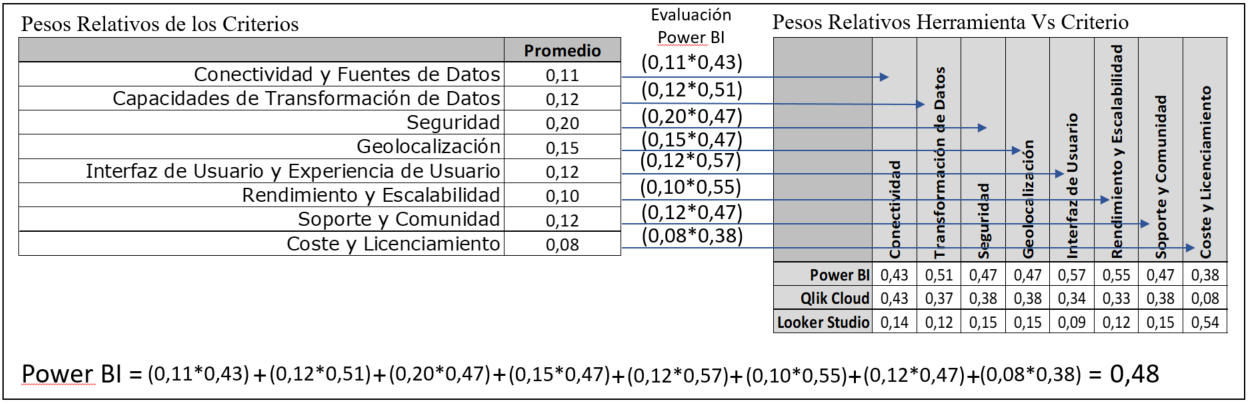
\includegraphics[width=6.25in]{media 2/image47} 

}

\caption{Calculo puntuación Global}\label{fig:unnamed-chunk-54}
\end{figure}

\hypertarget{resultados}{%
\subsubsection{Resultados}\label{resultados}}

Aplicando el método jerárquico AHP, se evaluaron tres herramientas de visualización de datos: Power BI, Qlik Cloud y Looker Studio. Los resultados finales posicionan a Power BI como la herramienta más adecuada para la implementación de los KPIs para le gestión de mantenimiento en la industria petrolera, con una puntuación de 0.48, seguida por Qlik Cloud con 0.35 y Looker Studio con 0.17. continuación, se detallan las conclusiones derivadas de esta evaluación.

\begin{table}[H]

\caption{\label{tab:unnamed-chunk-55}Matriz Pesos Promedio Criterios Vs Herramientas Visualización}
\centering
\fontsize{12}{14}\selectfont
\begin{tabular}[t]{l|r|r|r}
\hline
Categoria & Power\_BI & Qlik\_Cloud & Looker\_Studio\\
\hline
Conectividad y Fuentes de Datos & 0.05 & 0.05 & 0.02\\
\hline
Capacidades de Transformación de Datos & 0.06 & 0.05 & 0.02\\
\hline
Seguridad & 0.09 & 0.07 & 0.03\\
\hline
Geolocalización & 0.07 & 0.06 & 0.02\\
\hline
Interfaz de Usuario y Experiencia de Usuario & 0.07 & 0.04 & 0.01\\
\hline
Rendimiento y Escalabilidad & 0.05 & 0.03 & 0.01\\
\hline
Soporte y Comunidad & 0.06 & 0.05 & 0.02\\
\hline
Coste y Licenciamiento & 0.03 & 0.01 & 0.05\\
\hline
Total & 0.48 & 0.35 & 0.17\\
\hline
\end{tabular}
\end{table}

\hypertarget{conclusiones}{%
\section{CONCLUSIONES}\label{conclusiones}}

\hypertarget{power-bi-0.48}{%
\subsection{Power BI (0.48)}\label{power-bi-0.48}}

\begin{itemize}
\item
  \textbf{Funcionalidad y Características}: Se destaca por su amplia variedad de funcionalidades y características avanzadas. Su capacidad de integración con múltiples fuentes de datos, su flexibilidad en la creación de dashboards interactivos y sus robustas opciones de análisis.
  Conectividad y Transformación de Datos: Ofrece excelentes capacidades de conectividad y herramientas de transformación de datos (Power Query, Lenguaje M y DAX), lo cual facilita la preparación, limpieza y transformación de los datos.
\item
  \textbf{Rendimiento y Escalabilidad}: Maneja grandes volúmenes de datos de manera eficiente y escala bien con el crecimiento de las necesidades empresariales.
\item
  \textbf{Seguridad y Compliance}: Cuenta con sólidas características de seguridad, incluyendo la capacidad de restringir el acceso a datos específicos mediante roles y reglas DAX, y está bien alineado con los estándares de compliance.
\item
  \textbf{Costo}: Su modelo de licenciamiento es competitivo, ofreciendo opciones escalables para diferentes tamaños de empresas, desde la versión gratuita es una herramienta muy sólida en para el desarrollo de visualizaciones y el análisis de la información resultante del procesamiento de los datos maximizando así el valor de costo beneficio.
\end{itemize}

\hypertarget{qlik-cloud-0.35}{%
\subsection{Qlik Cloud (0.35)}\label{qlik-cloud-0.35}}

\begin{itemize}
\item
  \textbf{Funcionalidad y Características}: Es potente en análisis asociativo, permitiendo conexiones dinámicas entre datos. Puede no ser tan intuitivo como Power BI para usuarios inexpertos.
\item
  \textbf{Conectividad y Transformación de Datos}: Excelente en conectividad con una amplia gama de fuentes de datos y buenas capacidades de transformación de datos.
\item
  \textbf{Rendimiento y Escalabilidad}: Ofrece un rendimiento robusto y escalable, aunque puede requerir una curva de aprendizaje más pronunciada.
\item
  \textbf{Seguridad}: Ofrece características de seguridad robustas y es adecuado para cumplir con requisitos que demandan las leyes, aunque su gestión puede ser menos intuitiva que en Power BI.
\item
  \textbf{Costo}: El costo puede ser alto en comparación con Power BI o Looker Studio especialmente para organizaciones pequeñas.
\end{itemize}

\hypertarget{looker-studio-0.17}{%
\subsection{Looker Studio (0.17)}\label{looker-studio-0.17}}

\begin{itemize}
\item
  \textbf{Funcionalidad y Características}: Potente en su enfoque de modelado de datos sin embargo puede ser menos intuitivo y más limitado en términos de funcionalidades y flexibilidad en las visualizaciones en comparación con Power BI y Qlik Cloud.
\item
  \textbf{Conectividad y Transformación de Datos}: Buena capacidades de conectividad, la transformación de datos puede ser menos flexible sin un lenguaje robusto de consulta como DAX que implementa Power BI o el motor asociativo de Qlik.
\item
  \textbf{Rendimiento y Escalabilidad}: Enfrenta limitaciones de rendimiento y escalabilidad, especialmente con grandes volúmenes de datos, la velocidad de la red influye significativamente en el rendimiento tanto en el diseño como en la consulta de las visualizaciones.
\item
  \textbf{Seguridad}: Características de seguridad adecuadas no son tan robustas y configurables en comparación con Power BI y Qlik Cloud.
  Costo: Muy competitivo si se compara con sus contra partes Power BI y Qlik Cloud, sin embargo, esto no compensa las limitaciones en funcionalidad y rendimiento en empresas que necesiten capacidades avanzadas de análisis y visualización.
\end{itemize}

\hypertarget{conclusiuxf3n-final}{%
\section{Conclusión Final}\label{conclusiuxf3n-final}}

La aplicación del método jerárquico AHP en el contexto planteado para el caso práctico muestra que Power BI es la Herramienta de Visualización más adecuada para la implementación de los KPIs para la gestión de mantenimiento, gracias a su combinación superior de funcionalidad, conectividad, rendimiento, escalabilidad, seguridad y costo. Qlik Cloud sigue siendo una opción fuerte con capacidades robustas, especialmente en análisis asociativo, pero con una curva de aprendizaje más pronunciada y un costo potencialmente más alto. Looker Studio, aunque útil, es menos competitivo en este entorno específico debido a sus limitaciones en funcionalidad y rendimiento con grandes volúmenes de datos.

El método jerárquico AHP proporciona un marco robusto y flexible para evaluar y seleccionar la mejor herramienta de visualización en función del contexto específico. Su capacidad para manejar la subjetividad y la incertidumbre, considerar múltiples criterios simultáneamente y adaptarse a diferentes contextos lo convierte en una opción interesante y efectiva para abordar este tipo de problemas de decisión.

\printbibliography

\end{document}
